%\documentclass[•]{•}10pt,conference,compsocconf,letterpaper]{IEEEtran}
\documentclass[11pt,pdftex,a4paper]{article}%
\pdfoutput=1
%\documentclass{sig-alt-release2}
%\documentclass{llncs}
%\usepackage{llncsdoc}
\usepackage{verbatim}
\usepackage{amssymb}
\usepackage{lipsum}
\usepackage{multicol}
\usepackage{amsmath}
\usepackage{framed}
\usepackage{float}
\floatstyle{boxed} 
\restylefloat{figure}
\usepackage{subfig}
%\usepackage{mdframed}
\usepackage{amsthm}
\usepackage{tikz}
\usepackage{hyperref}
\usepackage{color}
\usepackage{soul}
\usepackage{tabularx}
%\usepackage{fullpage}
\usepackage{enumitem}
\setlist{nolistsep}
%\setenumerate{itemsep=0pt}
\usepackage{tikz}
\usepackage[margin=0.96in]{geometry}
\usepackage{cite}
\usepackage[textsize=tiny]{todonotes}
\usepackage{cleveref}
%\usepackage[dvips]{graphicx}
%\ifx\pdftexversion\undefined
%\usepackage[dvips]{graphicx}
%\else
%  \usepackage[pdftex]{graphicx}
%  \DeclareGraphicsRule{*}{mps}{*}{}
%\fi
\newif\ifcode
\codefalse
%%%
% comment this if you do not have
% algpseudocode package for algorithms.
\codetrue
%%%
\usepackage{macros}
\ifcode
\usepackage[ruled]{algorithm}
\usepackage{algpseudocode}
\usepackage{ioa_code}

%%%%%%%%%%%%%%%%%%%%%%%%%%%%%%%%%%%%%%%%%%%%%%%%%%%%%%%%%%%%%%%%%%%%%%%%%=
%%%%%%%%%%%%%%%%%%%%%%%%%%
%pour avoir plus de place
% \topmargin 0pt
% \advance \topmargin by -\headheight
% \advance \topmargin by -\headsep
% \textheight 8.9in
% \oddsidemargin 0pt
% \evensidemargin \oddsidemargin
% \marginparwidth 0.5in
% \textwidth 6.5in
% \setlength{\baselineskip}{13.2pt} % standard value is 13.75pt
\def\algofont{\footnotesize} %fonte pour les algos
%\interfootnotelinepenalty=10
%fin de pour avoir plus de place
%du coup il faut commenter la suite
%\textwidth 130mm
%\textheight 215mm
%jusqu'ici
%\renewcommand{\baselinestretch}{1.5}

%%%%%%%%%%%%%%%%%%%%%%%%%%%%%%%%%%%%%%%%%%%%%%%%%%%%%%%%%%%%%%%%
% Definitions
%%%%%%%%%%%%%%%%%%%%%%%%%%%%%%%%%%%%%%%%%%%%%%%%%%%%%%%%%%%%%%%%

\newtheorem{theorem}{Theorem}
%\newtheorem{reptheorem}[]{Theorem \ref{th:sl}}
%\newreptheorem{theorem}{Theorem}
\newtheorem{axiom}[theorem]{Axiom}
\newtheorem{case}[theorem]{Case}
\newtheorem{claim}[theorem]{Claim}
\newtheorem{proposition}{Proposition}
\newtheorem{explanation}[theorem]{Explanation}
\newtheorem{remark}[theorem]{Remark}
\newtheorem{fact}[theorem]{Fact}
% \newtheorem{conclusion}[theorem]{Conclusion}
% \newtheorem{condition}[theorem]{Condition}
\newtheorem{conjecture}[theorem]{Conjecture}
\newtheorem{corollary}[theorem]{Corollary}
% \newtheorem{criterion}[theorem]{Criterion}
\newtheorem{definition}{Definition}
% \newtheorem{exercise}[theorem]{Exercise}
\newtheorem{lemma}[theorem]{Lemma}
% \newtheorem{notation}[theorem]{Notation}
% \newtheorem{problem}[theorem]{Problem}
%\newtheorem{proposition}[theorem]{Proposition}
% \newtheorem{remark}[theorem]{Remark}
% \newtheorem{solution}[theorem]{Solution}
% \newtheorem{summary}[theorem]{Summary}
\newtheorem{observation}[theorem]{Observation}
%\newenvironment{proof}[1][Proof]{\noindent\textbf{#1.} }{\hfill $\Box$\\[2mm]} %\rule{0.5em}{0.5em}\\}
\newenvironment{proofsketch}[1][Proof sketch]{\noindent\textbf{#1.} }{\hfill $\Box$\\[2mm]} %\rule{0.5em}{0.5em}\\}

\newenvironment{reptheorem}[1][Theorem]{\noindent\textbf{#1}}{}
\def\lf{\tiny}
\def\rrnnll{\setcounter{linenumber}{0}}
\def\nnll{\refstepcounter{linenumber}\lf\thelinenumber}
\newcounter{linenumber}
\newenvironment{algorithmfig}{\hrule\vskip 3mm}{ \vskip 3mm \hrule }

\def\P{\ensuremath{\mathcal{P}}}
\def\DP{\ensuremath{\Diamond\mathcal{P}}}
\def\DS{\ensuremath{\Diamond\mathcal{S}}}
%\def\T{\ensuremath{\mathcal{T}}}
\def\Time{\mathbb{T}}
\def\S{\ensuremath{\mathcal{S}}}
\def\D{\ensuremath{\mathcal{D}}}
\def\W{\ensuremath{\mathcal{W}}}
\def\A{\ensuremath{\mathcal{A}}}
\def\B{\ensuremath{\mathcal{B}}}
\def\F{\ensuremath{\mathcal{F}}}
\def\R{\ensuremath{\mathcal{R}}}
\def\N{\ensuremath{\mathcal{N}}}
\def\I{\ensuremath{\mathcal{I}}}
\def\O{\ensuremath{\mathcal{O}}}
\def\Q{\ensuremath{\mathcal{Q}}}
\def\K{\ensuremath{\mathcal{K}}}
\def\L{\ensuremath{\mathcal{L}}}
\def\M{\ensuremath{\mathcal{M}}}
\def\V{\ensuremath{\mathcal{V}}}
\def\E{\ensuremath{\mathcal{E}}}
\def\C{\ensuremath{\mathcal{C}}}
\def\T{\ensuremath{\mathcal{T}}}
\def\X{\ensuremath{\mathcal{X}}}
\def\Y{\ensuremath{\mathcal{Y}}}
\def\Nat{\ensuremath{\mathbb{N}}}
\def\Om{\ensuremath{\Omega}}
\def\ve{\varepsilon}
\def\fd{failure detector}
\def\cfd{\ensuremath{?\P+\DS}}
\def\afd{timeless}
\def\env{\ensuremath{\mathcal{E}}}
%\def\faulty{unreliable}
\def\bounded{one-shot}
\def\cons{\textit{cons}}
\def\val{\textit{val}}
\def\code{\textit{code}}

\def\HSS{\mathit{h}}
\def\argmin{\mathit{argmin}}
\def\proper{\mathit{proper}}
\def\content{\mathit{content}}
\def\Level{\mathit{L}}
\def\Blocked{\mathit{Blocked}}
\def\Set{\mathit{Set}}
\def\TS{\mathit{TS}}
\def\shared{\mathit{shared}}
\def\exclusive{\mathit{exclusive}}

\newcommand{\correct}{\mathit{correct}}
\newcommand{\RNum}[1]{\uppercase\expandafter{\romannumeral #1\relax}}
\newcommand	{\faulty}{\mathit{faulty}}
\newcommand{\infi}{\mathit{inf}}
\newcommand{\live}{\mathit{live}}
\newcommand{\true}{\mathit{true}}
\newcommand{\false}{\mathit{false}}
\newcommand{\stable}{\mathit{Stable}}
\newcommand{\setcon}{\mathit{setcon}}
\newcommand{\remove}[1]{}

\newcommand{\Wset}{\textit{Wset}}
\newcommand{\Rset}{\textit{Rset}}
\newcommand{\Dset}{\textit{Dset}}

%\newcommand{\parts}{\textit{parts}}
\newcommand{\txns}{\textit{txns}}

\newcommand{\Read}{\textit{read}}
\newcommand{\Write}{\textit{write}}
\newcommand{\TryC}{\textit{tryC}}
\newcommand{\TryA}{\textit{tryA}}
\newcommand{\ok}{\textit{ok}}

\newcommand{\trylock}{\textit{trylock}}
\newcommand{\multitrylock}{\textit{multi-trylock}}
\newcommand{\CAS}{\textit{CAS}}
\newcommand{\mCAS}{\textit{mCAS}}

\def\Nomega{\ensuremath{\neg\Omega}}
\def\Vomega{\ensuremath{\overrightarrow{\Omega}}}

\newcommand{\id}[1]{\mbox{\textit{#1}}}% for identifiers in code
\newcommand{\res}[1]{\mbox{\textbf{#1}}}% reserved words

\newcommand{\ignore}[1]{}

\definecolor{dkgreen}{rgb}{0,0.6,0}
\definecolor{gray}{rgb}{0.5,0.5,0.5}
\definecolor{mauve}{rgb}{0.58,0,0.82}


\definecolor{gpcolor}{rgb}{0.6,0.2,0.3}
\newboolean{showcomments}
\setboolean{showcomments}{true}
\ifthenelse{\boolean{showcomments}}
{ \newcommand{\mynote}[3]{
    \fbox{\bfseries\sffamily\scriptsize#1}
    {\small$\blacktriangleright$\textsf{\emph{\color{#3}{#2}}}$\blacktriangleleft$}}
}
{ 
\newcommand{\mynote}[3]{}}
\newcommand{\sr}[1]{\mynote{SR}{#1}{magenta}}


\begin{document}
\bibliographystyle{abbrv}

\title{The Cost of Concurrency in Hybrid Transactional Memory}
%%%%%%%%%%%%%%%%%%%%%%%%%%%%%%%%%%%%%%%%%%%%%%%%%%%%%%%%%%%%%%%%%%%%%%%%%%%%%%%%
\date{}
\maketitle
%
\thispagestyle{empty}
%
\begin{abstract}
The \emph{Transactional Memory (TM)} abstraction is a synchronization mechanism 
that allows the programmer to \emph{speculatively} execute sequences of shared-memory
operations as \emph{atomic transactions}.
Several TM designs are implemented entirely in software which typically incurs significant performance overhead.
Thus, current CPUs have included instructions to mark a block of memory accesses as transactional, allowing them to be executed \emph{atomically} in hardware.
However, hardware transactions may be spuriously aborted due to several reasons: cache capacity overflows, interrupts etc., thus leading to \emph{hybrid} TMs 
in which the \emph{fast} hardware transactions are complemented with \emph{slower} software transactions that do not experience spurious aborts.
To allow hardware transactions in a HyTM to detect conflicts with software transactions, hardware transactions must be \emph{instrumented} to perform additional metadata accesses, which introduces overhead.

In this paper, we identify the \emph{cost of concurrency} in HyTMs by presenting two provably \emph{opaque} HyTM algorithms in which both hardware and software transactions perform an optimal number of metadata accesses.
The first algorithm is \emph{progressive}: a transaction may be aborted only due to a \emph{data} conflict with a concurrent transaction.
The second algorithm is progressive only for \emph{read-only} software transactions.
We show how some of the metadata accesses in these algorithms can be performed \textit{non-speculatively} without violating opacity.
This has the potential to reduce conflict aborts in hardware.
We evaluate implementations of these algorithms on Intel Haswell, which does not support non-speculative accesses inside a hardware transaction, and the IBM Power8 processor, which does.
Viewed collectively, our results highlight the subtle performance tradeoffs between concurrency, instrumentation cost and the complexity of software transactions in the design space of hybrid TMs.
\end{abstract}

\newpage

%\newpage
\pagenumbering{arabic}\setcounter{page}{1}

%!TEX root = htm.tex
\section{Introduction}
\label{sec:intro}
%
%
The \emph{Transactional Memory (TM)} abstraction is a synchronization mechanism 
that allows the programmer to \emph{optimistically} execute sequences of shared-memory
operations as \emph{atomic transactions}.
Several software TM designs~\cite{norec, ST95,HLM+03, astm, fraser} have been introduced subsequent to the original TM proposal based in
hardware~\cite{HM93}. 
The original dynamic STM implementation DSTM~\cite{HLM+03} ensures that a transaction aborts only if there is a read-write \emph{data conflict} with a concurrent
transaction (\`a la \emph{progressiveness}~\cite{tm-book}). However, read operations in DSTM must \emph{incrementally} validate
the responses of all previous read operations to avoid inconsistent executions. 
This results in quadratic  (in the size of the transaction's read
set) step-complexity for transactions. Subsequent STM 
implementations like NOrec~\cite{norec} and TL2~\cite{DSS06}
minimize the impact on performance due to incremental validation.
NOrec uses a global sequence lock that is read at the start of a transaction and performs \emph{value-based}
validation during read operations only if the value of the global lock has been changed (by an updating transaction) 
since reading it.
TL2, on the other hand, eliminates incremental validation completely.
Like NOrec, it uses a global sequence lock, but each data item also 
has an associated sequence lock value that is updated alongside the data item.
When a data item is read, if its associated sequence lock value is different 
from the value that was read from the sequence lock at the start of the transaction, then the transaction aborts.

In fact, STMs like TL2 and NOrec ensure progress in the absence of data conflicts with 
O(1) step complexity read operations and \emph{invisible reads} (read operations which 
do not modify shared memory) 
Nonetheless, TM designs that are implemented entirely in software still incur significant performance overhead.
Thus, current CPUs have included instructions to mark a block of memory accesses as transactional~\cite{Rei12, asf, bluegene}, allowing them to be executed \emph{atomically} in hardware.
Hardware transactions promise better performance than STMs, but they offer no progress guarantees 
since they may experience \emph{spurious} aborts. This motivates the need for
\emph{hybrid} TMs in which the \emph{fast} hardware transactions are 
complemented with \emph{slower} software transactions that do not have spurious aborts.

To allow hardware transactions in a HyTM to detect conflicts with software transactions, they must be \emph{instrumented} to perform additional metadata accesses, which introduces overhead.
Hardware transactions typically provide automatic conflict detection at cacheline granularity,
thus ensuring that the transaction itself will be aborted if it experiences memory contention on the cacheline.
This is at least the case with Intel's Transactional Synchronization Extensions~\cite{haswell}.
The IBM POWER8 ISA additionally allows hardware transactions to access metadata \emph{non-speculatively}, 
thus bypassing automatic conflict detection. While this has the advantage of potentially reducing contention aborts
in hardware, this makes the design of HyTM implementations potentially harder to prove correct.

In \cite{htmdisc15}, it was shown that hardware transactions in progressive HyTMs must perform
at least one metadata access per transactional read and write.
In this paper, we show that in progressive HyTMs with invisible reads, 
software transactions \textit{cannot} avoid incremental validation.
Specifically, we prove that \textit{each read operation} of a software transaction in a progressive HyTM
must necessarily incur a validation cost that is \emph{linear} 
in the size of the transaction's read set. 
This is in contrast to TL2 which is progressive and has constant complexity read operations.
Thus, in addition to the linear instrumentation cost in hardware transactions, there is a quadratic step complexity cost in software transactions.

We then present \emph{opaque} HyTM algorithms providing \emph{progressiveness for a subset of transactions} that are  %both hardware and software transactions \trevor{maybe just ``transactions''?}
optimal in terms of hardware instrumentation.
Algorithm~1 is progressive for all transactions, but it incurs high instrumentation overhead in practice.
Algorithm~2 avoids all instrumentation in fast-path read operations, but is progressive only for slow-path reading transactions.
We also sketch how \emph{some} hardware instrumentation can be performed \textit{non-speculatively} without violating opacity.

We performed experiments comparing our HyTM algorithms to TL2, Transactional Lock Elision (TLE) and Hybrid NOrec~\cite{hynorecriegel} 
using a binary search tree microbenchmark.
In these experiments, we studied two types of workloads: workloads in which essentially all transactions commit on the fast-path, 
and workloads in which some thread periodically performs transactions on the slow-path.
Our experiments with Intel and IBM Power8 HTMs   
seem to suggest that (i) the \emph{cost of concurrency} also exists in practice; high hardware instrumentation impacts performance negatively on Intel and even more so on POWER8 due to its limited transactional
cache capacity, (ii) 
it is important to build HyTMs that provide progressiveness for a maximal set of transactions, but reducing fast-path instrumentation
without using global contending bottlenecks and (iii) 
there is no easy to way to derive more efficient HyTMs by taking advantage of non-speculative accesses supported within the fast-path in POWER8 processors
(but not in Intel HTMs).
%We explore the concurrency vs. hardware instrumentation vs. software validation tradeoffs for these algorithms.
%Preliminary experiments on Intel Haswell (resp. IBM Power 8) not supporting (resp. supporting) non-speculative accesses inside hardware,
%seem to suggest that the inherent \emph{cost to concurrency} in HyTMs also exists in practice and discuss algorithmic techniques to overcome them.

\vspace{1mm}\noindent\textbf{Roadmap.}
\cref{sec:hytm} presents details of the HyTM model that extends the model introduced in \cite{htmdisc15}.
\cref{sec:lb} presents our main lower bound result on the step-complexity of slow-path transactions in progressive HyTMs
while \cref{sec:hytmalgos} presents opaque HyTMs that are progressive for a subset of transactions.
\cref{sec:eval} presents results from experiments on Intel Haswell and IBM POWER8 architectures which provide a clear characterization of the cost
of concurrency in HyTMs as well as the ability to use direct accesses within hardware transactions.
\cref{sec:rel} presents the related work along with concluding remarks. Formal proofs and pseudocodes are provided in the Appendix.
%
%
%!TEX root = htm.tex
\section{Hybrid transactional memory (HyTM)}
\label{sec:hytm}
%
In this section, we adopt the formal model of HyTMs originally proposed in \cite{htmdisc15}.

\vspace{1mm}\noindent\textbf{Transactional memory (TM).} 
A \emph{transaction} is a sequence of \emph{transactional operations}
(or \emph{t-operations}), reads and writes, performed on a set of \emph{transactional objects} 
(\emph{t-objects}). 
A TM \emph{implementation} provides a set of
concurrent \emph{processes} with deterministic algorithms that implement reads and
writes on t-objects using  a set of \emph{base objects}.
% More precisely, for each transaction $T_k$, a TM implementation must support the following t-operations: 
% $\mathit{read}_k(X)$, where $X$ is a t-object, that returns a value in
% a domain $V$
% or a special value $A_k\notin V$ (\emph{abort}),
% $\mathit{write}_k(X,v)$, for a value $v \in V$,
% that returns $\mathit{ok}$ or $A_k$, and
% $\mathit{tryC}_k$ that returns $C_k\notin V$ (\emph{commit}) or $A_k$.
% Additionally, we assume that a transaction $T_k$
% may perform a $\mathit{start_k}$ that is the first t-operation performed by $T_k$ prior to invoking any $\mathit{read}_k$ or $\mathit{write}_k$.

\vspace{1mm}\noindent\textbf{Configurations and executions.} 
A \emph{configuration} of a TM implementation specifies the state of each base object and each process. 
In the \emph{initial} configuration, each base object has its initial value and each process is in its initial state. 
An \emph{event} (or \emph{step}) of a transaction invoked by some process is an invocation of a t-operation, 
a response of a t-operation, or an atomic \emph{primitive} operation applied to base object along with its response. 
%An event $e$ is \emph{applicable} to a configuration $C$ if $e$ can legally be applied to $C$. 
%Applying an event $e$ to a configuration $C$ results in another configuration $C' = e(C)$.
An \emph{execution fragment} is a (finite or infinite) sequence of events $E = e_1,e_2,\dots$. 
%$E$ is applicable to a configuration $C$ if $e_1$ is applicable to $C$, $e_2$ is applicable to $e_1(C)$, 
%and so forth. 
An \emph{execution} of a TM implementation $\mathcal{M}$ is an
execution fragment where, informally, each event respects the
specification of base objects and the algorithms specified by $\mathcal{M}$.

We consider the dynamic programming model: the \emph{read set} (resp., the \emph{write set}) of a transaction $T_k$ in an execution $E$,
denoted $\Rset_E(T_k)$ (resp., $\Wset_E(T_k)$), is the set of t-objects that $T_k$ attempts to read (and resp. write) 
by issuing a t-read (resp., t-write) invocation in $E$ (for brevity, we sometimes 
omit the subscript $E$ from the notation).

For any finite execution $E$ and execution fragment $E'$, $E\cdot E'$ denotes the concatenation of $E$ and $E'$,
and we say that $E\cdot E'$ is an \emph{extension}
of $E$.
%Let $E$ be an execution fragment.
For every transaction identifier $k$,
$E|k$ denotes the subsequence of $E$ restricted to events of
transaction $T_k$.
% If $E|k$ is non-empty,
% we say that $T_k$ \emph{participates} in $E$,
Let $\txns(E)$ denote the set of transactions that participate in $E$.
Two executions $E$ and $E'$
are \emph{indistinguishable} to a set $\mathcal{T}$ of transactions, if
for each transaction $T_k \in \mathcal{T}$, $E|k=E'|k$.
A transaction $T_k\in \txns(E)$ is \emph{complete in $E$} if
$E|k$ ends with a response event.
The execution $E$ is \emph{complete} if all transactions in $\txns(E)$
are complete in $E$.
A transaction $T_k\in \txns(E)$ is \emph{t-complete} if $E|k$
ends with $A_k$ or $C_k$; otherwise, $T_k$ is \emph{t-incomplete}.

We assume that base objects are accessed with \emph{read-modify-write} (rmw) primitives. 
A rmw primitive event on a base object is \emph{trivial} if, in any configuration, its application
does not change the state of the object. 
Otherwise, it is called \emph{nontrivial}.
Events $e$ and $e'$ of an execution $E$  \emph{contend} on a base
object $b$ if they are both primitives on $b$ in $E$ and at least 
one of them is nontrivial.

\vspace{1mm}\noindent\textbf{Hybrid transactional memory executions.}
We now describe the execution model of a \emph{Hybrid transactional memory (HyTM)} implementation.
In our HyTM model, shared memory configurations may be modified by accessing base objects via two kinds of
primitives: \emph{direct} and \emph{cached}.
(i) In a direct access, the rmw primitive operates on the memory state:
the direct-access event atomically reads the value of the object in
the shared memory and, if necessary, modifies it.
(ii) In a cached access performed by a process $i$, the rmw primitive operates on the \emph{cached}
state recorded in process $i$'s \emph{tracking set} $\tau_i$. 

More precisely, $\tau_i$ is a set of triples $(b, v, m)$ where $b$ is a base object identifier, $v$ is a value, 
and $m \in \{\shared, \exclusive\}$ is an access \emph{mode}. 
The triple $(b, v, m)$ is added to the tracking set when $i$ performs a cached
rmw access of $b$, where $m$ is set to $\exclusive$ if the access is
nontrivial, and to $\shared$ otherwise.  
We assume that there exists some constant $\TS$
such that the condition $|\tau_i| \leq \TS$ must always hold; this
condition will be enforced by our model.
A base object $b$ is \emph{present} in $\tau_i$ with mode $m$ if $\exists v, (b,v,m) \in \tau_i$.

Any transaction $T_k \in \ms{txns}(E)$ that performs at least one cached access necessarily performs a \emph{cache-commit} primitive as the last event of $E|k$ if it has already not terminated before. 
A \emph{cache-commit} primitive issued by process $i$ with
a valid $\tau_i$ does the following: for each base object $b$ such that $(b,v,\exclusive) \in \tau_i$, the value of $b$ in $C$ is updated to $v$. 
Finally, $\tau_i$ is set to $\emptyset$ and the primitive 
returns $\textit{commit}$. 
% A trivial (resp.\ nontrivial) 
% cached primitive $\langle g,h \rangle$ applied to $b$ 
% by process $i$ 
% checks whether $b$ is present in exclusive
% (resp.\ any) mode in $\tau_j$ 
% for any $j\neq i$. If so, $\tau_i$ is set to $\emptyset$ and the
% primitive returns $\bot$. 
% %
% Otherwise, the triple $(b, v, \shared)$ (resp. $(b, g(v), \exclusive)$)
% is added to $\tau_i$,  where $v$ is the most recent cached value of $b$ in $\tau_i$
% (in case $b$ was previously accessed by $i$ within the current
% hardware transaction) or the value of $b$ in the current
% memory configuration, and finally $h(v)$ is returned.
%

\vspace{1mm}\noindent\textbf{Hardware aborts.}
A tracking set can be \emph{invalidated} by a concurrent process: 
if, in a configuration $C$ where  $(b,v,\exclusive)\in\tau_i$
(resp., $(b,v,\shared)\in\tau_i)$,  a process $j\neq i$ applies any primitive 
(resp., any \emph{nontrivial} primitive) to $b$, then $\tau_i$ becomes
\emph{invalid} and any subsequent event invoked by $i$
sets $\tau_i$ to $\emptyset$ and returns $\bot$. We refer to this event as a \emph{tracking set abort}.

Any transaction that performs at least one cached access must necessarily perform a \emph{cache-commit} primitive 
that determines the terminal response of the transaction.
A cache-commit primitive
issued by process $i$ with
a valid $\tau_i$ does the following: for each base object $b$ such that $(b,v,\exclusive) \in \tau_i$, the value of $b$ in $C$ is updated to $v$. 
Finally, $\tau_i$ is set to $\emptyset$ and the operation returns $\textit{commit}$. 
We assume that a fast-path transaction $T_k$ returns $A_k$
as soon an underlying cached primitive or \emph{cache-commit} returns $\bot$.

\vspace{1mm}\noindent\textbf{Slow-path and fast-path transactions.}
We partition HyTM transactions into \emph{fast-path transactions} and \emph{slow-path transactions}.
A slow-path transaction models a regular software transaction.
An event of a slow-path transaction is either an invocation or response of a t-operation, or
a direct rmw primitive on a base object. 
A fast-path transaction essentially encapsulates a hardware transaction. Specifically, in any execution $E$,
we say that a transaction $T_k\in \ms{txns}(E)$ is a fast-path transaction if $E|k$ contains at least one cached event.
An event of a \emph{hardware transaction} includes series of direct trivial accesses and at least one cached access
followed by a cache-commit primitive.

Concretely, the HyTM model provides automatic detection of contending accesses for fast-path transactions:
%
\begin{remark}[Tracking set aborts]
\label{re:traborts}
%
Let $T_k \in \ms{txns}(E)$ be any t-incomplete transaction executed by process $i$, 
where $(b,v,\exclusive)\in\tau_i$ (resp., $(b,v,\shared)\in\tau_i$) after execution $E$, and $e$ be any event (resp., nontrivial event) 
that some process $j\neq i$ is poised to apply after $E$.
The next event of $T_k$ in any extension of $E\cdot e$ is $A_k$.
%
%For any t-incomplete transaction $T_k \in \ms{txns}(E)$ executed by process $i$ and $(b,v,\exclusive)\in\tau_i$ (and resp. $(b,v,\shared)\in\tau_i$) after execution $E$
%and let $e$ be any event (and resp. nontrivial event) that some process $j\neq i$ is poised to apply after $E$, then the next event of $T_k$ in any extension of $E\cdot e$
%is $A_k$.
\end{remark}
%
We also assume that there is a constant $\TS$ such that the condition $|\tau_i| \leq \TS$ must always hold.
%
\begin{remark}[Capacity aborts]
\label{re:capacity}
Any cached access performed by a process $i$ first checks the condition $|\tau_i|=\TS$, where $\TS$ is a pre-defined constant, and if so, it
sets $\tau_i=\emptyset$ and immediately returns $\bot$. 
\end{remark}

\vspace{1mm}\noindent\textbf{Direct reads within fast-path.}
Note that we specifically allow hardware transactions to perform reads without adding the corresponding base object to
the process's tracking set, thus modelling the \emph{suspend/resume} instructions supported by 
IBM Power8 architectures. Note that Intel's HTM does not support this feature: an event of a fast-path transaction
does not include any direct access to base objects.

%
\vspace{1mm}\noindent\textbf{HyTM properties.}
%\trevor{reading here}
Throughout this paper, we consider the TM-correctness property of \emph{opacity}~\cite{tm-book}: an execution
$E$ is opaque if there exists a \emph{legal} sequential execution $S$ equivalent to some t-completion of $E$
that respects the \emph{real-time ordering} of transactions in $E$.

We also assume a weak \emph{TM-liveness} property for t-operations in this paper: every t-operation returns a matching
response within a finite number of its own steps if running step-contention free from a \emph{quiescent} configuration,
\emph{i.e.}, a configuration in which every transaction is t-complete.

Algorithms and lower bounds presented in this paper concern HyTMs that provide \emph{invisible reads}: t-read operations do not perform
nontrivial primitives in any execution.
%
%
% \begin{figure*}[!ht]
% \begin{center}
% 	\subfloat[\label{sfig:ob-01}]{\scalebox{0.5}[0.5]{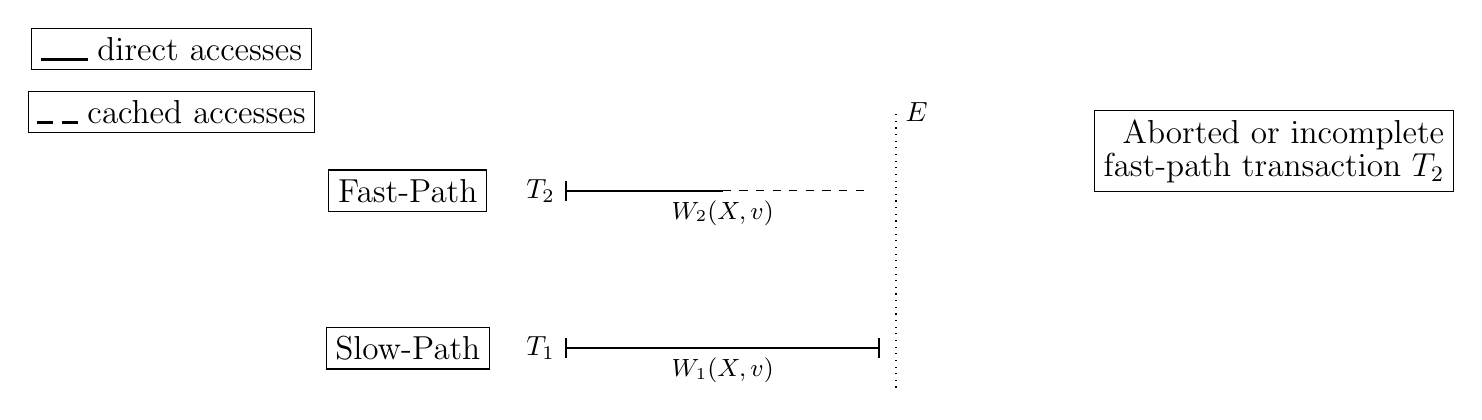
\begin{tikzpicture}
\node (w2) at (10,0) [] {};
\node (w1) at (10,-2) [] {};
\node (w3) at (18,-2) [] {};


\draw (w2) node [below] {\small {$W_2(X,v)$}};

\draw (w1) node [below] {\small {$W_1(X,v)$}};
%\draw (w1) node [below] {\tiny {$T_1$ commits}};

\node[draw,align=left] at (6,0) {{\large Fast-Path}};
\node[draw,align=left] at (6,-2) {{\large Slow-Path}};

\begin{scope}   
\draw [|-,thick] (8,0) node[left] {$T_2$} to (10,0);
\draw [-,dashed] (10,0) to (11.8,0);
\draw [|-|,thick] (8,-2) node[left] {$T_1$} to (12,-2);
\draw [-,dotted] (12.2,-2.5)  to (12.2,1) node[right] {$E$};
\end{scope}
%
\node[draw,align=right] at (17,.5) {\large {Aborted or incomplete}\\ {\large fast-path transaction $T_2$}};
%
\node[draw,align=right] at (3,1.8) {\rule{6mm}{1pt} \large {direct accesses}};
\node[draw,align=right] at (3,1) {\rule{2mm}{1pt} \rule{2mm}{1pt} \large{cached accesses}};

%
\end{tikzpicture}
}}
% 	\hspace{10mm}
% 	\subfloat[\label{sfig:ob-02}]{\scalebox{0.5}[0.5]{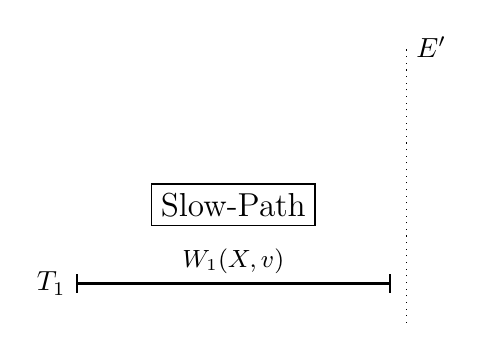
\begin{tikzpicture}

\node (w1) at (11,-2) [] {};


\draw (w1) node [above] {\small {$W_1(X,v)$}};
%\draw (w1) node [below] {\tiny {$T_1$ commits}};

\node[draw,align=left] at (11,-1) {{\large Slow-Path}};

\begin{scope}   
\draw [|-|,thick] (9,-2) node[left] {$T_1$} to (13,-2);
\draw [-,dotted] (13.2,-2.5)  to (13.2,1) node[right] {$E'$};
\end{scope}
%
%
\end{tikzpicture}
}}
% 	 
% \end{center}
% \caption{
% \label{fig:ob1}
% Execution $E$ in Figure~\ref{sfig:ob-01} is indistinguishable
% to $T_1$ from the execution $E'$ in Figure~\ref{sfig:ob-02}}
% \end{figure*}
%

%
%!TEX root = htm.tex
\section{Hybrid transactional memory algorithms}\label{sec:hytmalgos}
%
%%%%%%%%%%%%%%%%%%%%%%%%%%%%%%%%%%%%%%%%%%%%%%%%
\begin{figure*}[!ht]
      
     \scalebox{.82}[.82]{
     \begin{tabularx}{\textwidth}{c|c|c|c|c}
%	\hline
	~~~~~ & Algorithm~\ref{alg:inswrite} & Algorithm~\ref{alg:inswrite2} & TLE & HybridNorec\\ \hline
	Instrumentation in fast-path reads & per-read & none & none & none \\ \hline
	Instrumentation in fast-path writes & per-write & per-write & constant & none \\ \hline
	Validation in slow-path reads & $\Omega(|Rset|)$ & $\Omega(|Rset|)$ & None & $\Omega(|Rset|)$ only if concurrency \\ \hline
	h/w-s/f concurrency & prog. & prog. for slow-path readers & zero & not prog., but small contention window \\ \hline
	Uncached accesses inside fast-path & yes & yes & no & yes \\ \hline
	opacity & yes & yes & Yes & Yes 
	%    \hline
   \end{tabularx}
\caption{Table summarizing complexities of HyTM implementations}\label{fig:main}    
}
\end{figure*}
%%%%%%%%%%%%%%%%%%%%%%%%%%%%%%%%%%%%%%%%%%%%%%%%%%%
%
In this section, we present progressive opaque HyTM algorithms that subject to the lower bound
of Theorem~\ref{th:impossibility} and then discuss some techniques to circumvent the lower bound.
%
%%%%%%%%%%%%%%%%%%%%%%%%%%%%%%%%%%%%%%%%%%%%%%%%%%%%%%%%%%%%%%%%%%%%%
%!TEX root = htm.tex
%%%%%%%%%%%%%%%%%%%%%%%%%%%%%%%%%%%%%%%%%%%%%%%%
\begin{algorithm}[!ht]
\caption{Progressive fast-path and slow-path opaque HyTM implementation; code for transaction $T_k$}
\label{alg:inswrite}
\begin{algorithmic}[1]
  	\begin{multicols}{2}
  	{
  	\footnotesize
	\Part{Shared objects}{
		\State $v_j$, value of each t-object $X_j$ 
		\State $r_{j}$, a versioned lock for each t-object $X_j$
	}\EndPart	
	\Statex
	\Part{Process local objects}{
		\State $\Rset(T_k)$, storing $\{X_j,r_j\}$
		\State $\Wset(T_k)$, storing $\{X_j, v_j\}$
	}\EndPart
	\Statex
	\textbf{Code for fast-path transactions}
	\Statex
	\Part{$\textit{read}_k(X_j)$}\quad\Comment{fast-path}{
		\State $\textit{ov}_j := \Read(v_j)$ \Comment{cached read} \label{line:lin1}
		\State $\textit{or}_j := \Read(r_j)$ \Comment{uncached read}
		\If{$\textit{or}_j$ $\mathrel{\&}1$}  \label{line:hread}
			\Return $A_k$ \EndReturn
		\EndIf
		
		\Return $\textit{ov}_j$ \EndReturn
		
   	 }\EndPart
	\Statex
	%\Comment{What is the best strategy to buffer writes?}
	\Part{$\textit{write}_k(X_j,v)$}{\quad\Comment{fast-path}
		\State $\textit{or}_j := \Read(r_j)$ \Comment{cached read}
		\If{$\textit{or}_j$ $\mathrel{\&} 1$}  		
			\Return $A_k$ \EndReturn
		\EndIf
		
		\State $\Write(r_j,\textit{or}_j+2)$ \Comment{uncached write}
		\State $\Write(v_j,v)$ \Comment{uncached write} 
		\Return $\ok$ \EndReturn
		
   	}\EndPart
	\Statex
	
	\Part{$\textit{tryC}_k$()}{\quad\Comment{fast-path}
		\State $\ms{commit-cache}_i$ \label{line:lin3} \Comment{returns $C_k$ or $A_k$}
  	 }\EndPart
  	 
  	 \Statex
  	\Part{Function: $\lit{release}(Q)$}{
  		\ForAll{$X_j \in Q$}	
 			\State $r_j.\lit{write}(or_j+1)$ \label{line:rel1}	
		\EndFor
		
	}\EndPart
 	\Statex
	\Part{Function: $\lit{acquire}(Q)$}{
  		\ForAll{$X_j \in Q$}	
 			\If{ $r_j.\lit{setV}()$} \label{line:acq1}
			  \State $\ms{Lset}(T_k):=\ms{Lset}(T_k)\cup \{X_j\}$
			  \Return $\true$ \EndReturn
			\EndIf
			\State $\lit{release}(\ms{Lset}(T_k))$
			\Return $\false$ \EndReturn
		\EndFor
		
	}\EndPart
	\Statex
	\Statex \Comment{Implement using LL/SC on Power8}
	\Part{Function: $\lit{setV}()$}{
% 		\State $\ms{success} \gets \lit{false}$
% 		
% 		\While{($\neg \ms{success}$)} \Comment {spin until we get the lock}
		%\State $\ms{or}_j \gets$ $r_j.\Read()$ $\mathrel{\&}1111...1110$
		\If{$r_j$.CAS($or_j$, $or_j+1$)} 
		  \Return $\false$  \EndReturn
		\EndIf
		\Return $\true$ \EndReturn
	}\EndPart
  	 
  	 \newpage
	\textbf{Code for slow-path transactions}
	\Statex
	\Part{\Read$_k(X_j)$}\quad\Comment{slow-path}{
		  \If{$X_j\in \Wset(T_k)$}
		    \Return $\Wset(T_k).\lit{locate}(X_j)$ \EndReturn
		  \Else
		  
		  \State $\textit{or}_j := \Read(r_j)$ \label{line:readorec}
		  \State $\textit{ov}_j := \Read(v_j)$ \label{line:read2}
		  \State $\Rset(T_k) := \Rset(T_k)\cup\{X_j,or_j\}$ \label{line:rset}
		  \If{$\textit{or}_j$ $\mathrel{\&} 1$} \label{line:abort0}	
			\Return $A_k$ \EndReturn
		  \EndIf
		 
		  \If{$\neg \lit{validate}()$} \label{line:valid}
			\Return $A_k$ \EndReturn
		  \EndIf
		  \EndIf
		  \Return $\textit{ov}_j$ \EndReturn
		
   	 }\EndPart
	\Statex
	\Part{\Write$_k(X_j,v)$}\quad\Comment{slow-path}{
		
			\State $\textit{or}_j := \Read(r_j)$
			\State $\textit{nv}_j := v$
			\If{$\textit{or}_j$ $\mathrel{\&} 1$}	
			\Return $A_k$ \EndReturn
			\EndIf
			\State $\Wset(T_k) := \Wset(T_k)\cup\{X_j,\textit{nv}_j\}$
			\Return $\ok$ \EndReturn
		
   	}\EndPart
	\Statex
	
	%\Statex	
	\Part{\TryC$_k$()}\quad\Comment{slow-path}{
		\If{$\Wset(T_k)= \emptyset$}
			\Return $C_k$ \EndReturn \label{line:return}
		\EndIf
		\If{$\lit{acquire}(\Wset(T_k))$}	\label{line:acq}
		
		\If{$\neq \lit{validate}()$} \label{line:abort3}
			\State $\lit{release}( \ms{Wset}(T_k))$ 
			\Return $A_k$ \EndReturn
		\EndIf
		\ForAll{$X_j \in \Wset(T_k)$}
	 		\State  $v_j.\lit{write}(\textit{nv}_j)$ \label{line:write}
			 
	 	\EndFor	
		  
		\State $\lit{release}(\Wset(T_k))$   \label{line:rel}	
   		\Return $C_k$ \EndReturn
   		\Else
		  \Return $A_k$ \EndReturn
		  \EndIf
   	 }\EndPart		
	 
 	
	\Statex
	\Part{Function: $\lit{validate}()$}{\quad\Comment{Validate slow-path reading transactions}
		\If{$\exists X_j \in Rset(T_k)$;$X_j \not\in \Wset(T_k)$:$(\textit{or}_j\neq \Read(r_j))$} \label{line:valid}
			\Return $\false$ \EndReturn
		  \EndIf
		 \Return $\true$ \EndReturn
	}\EndPart
		
  	 }
	\end{multicols}
  \end{algorithmic}
\end{algorithm}
%%%%%%%%%%%%%%%%%%%%%%%%%%%%%%%%%%%%%%%%%%%%%%%%
\begin{figure*}[!h]
      
     \scalebox{.9}[.9]{
     \begin{tabularx}{\textwidth}{c|c|c|c|c}
%	\hline
	~~~~~ & Algorithm~\ref{alg:inswrite} & Algorithm~\ref{alg:inswrite2} & TLE & HybridNorec\\ \hline
	Instrumentation in fast-path reads & per-read & none & none & none \\ \hline
	Instrumentation in fast-path writes & per-write & per-write & constant & none \\ \hline
	Validation in slow-path reads & $\Omega(|Rset|)$ & $\Omega(|Rset|)$ & None & $\Omega(|Rset|)$ only if concurrency \\ \hline
	h/w-s/f concurrency & prog. & prog. for slow-path readers & zero & not prog., but small contention window \\ \hline
	Uncached accesses inside fast-path & yes & yes & no & yes \\ \hline
	opacity & yes & yes & Yes & Yes 
	%    \hline
   \end{tabularx}
\caption{Table}\label{fig:main}    
}
\end{figure*}
%%%%%%%%%%%%%%%%%%%%%%%%%%%%%%%%%%%%%%%%%%%%%%%%%%%
\subsection{Instrumentation-optimal progressive HyTMs }
\label{sec:hytm1}
%
For every t-object $X_j$, our implementation maintains a base object $v_j\in \mathbb{D}$ that stores the value of $X_j$
and a \emph{sequence lock} $r_{j}$. The sequence lock is an unsigned integer whose LSB bit stores the \emph{locked} state.
Specifically, we say that process $p_i$ \emph{holds a lock on $X_j$ after an execution $E$} if
$\textit{or}_j$ $\mathrel{\&} 1=1$ after $E$, where $\textit{or}_j$ is the value of $r_j$ after $E$.

\vspace{1mm}\noindent\textit{Fast-path transactions:}
For a fast-path transaction $T_k$ executed by process $p_i$, the $\Read_k(X_j)$ implementation first reads $r_j$ (uncached)
and returns $A_k$ if some other process $p_j$ holds a lock on $X_j$.
Otherwise, it returns the value of $X_j$.
Updating fast-path transactions 
As with $\Read_k(X_j)$, the $\Write (X_j,v)$ implementation returns $A_k$ if some other process $p_j$ holds a lock on $X_j$.
Process $p_i$ then increments the value of $r_j$ by $2$ via a direct access and stores the cached state of $X_j$ along with its value $v$.
If the cache has not been invalidated, $p_i$ updates the shared memory
during $\TryC_k$ by invoking the $\ms{commit-cache}$ primitive.

\vspace{1mm}\noindent\textit{Slow-path read-only transactions:}
Any $\Read_k(X_j)$ invoked by a slow-path transaction first reads the value of the object from $v_j$, 
checks if $r_j$ is se, adds $r_j$ to $\Rset(T_k)$
and then performs \emph{validation} on its entire read set to check if any of them have been modified. 
If either of these conditions is true,
the transaction returns $A_k$. Otherwise, it returns the value of $X_j$. 
Validation of the read set is performed by re-reading the values of the sequence lock entires stored in $\Rset(T_k)$.
%A read-only transaction simply returns $C_k$ during the tryCommit.

\vspace{1mm}\noindent\textit{Slow-path updating transactions:}
% The $\Write_k(X,v)$ implementation of a slow-path transaction stores
% $v$ and the current value of $X_j$ locally, 
% deferring the actual update in shared memory to tryCommit. 
An updating slow-path transaction $T_k$ attempts to obtain exclusive write access to its 
entire write set by performing \emph{compare-and-set} (\emph{cas})
primitive that checks if the value of $r_j$, for each $X_j\in \Wset(T_k)$, is unchanged since last reading it during $\Write_k(X.v)$
If all the locks on the write set were acquired successfully, $T_k$ performs validation of the read set and returns $C_k$ if successful, else $p_i$ aborts the transaction.

\vspace{1mm}\noindent\textit{Non-cached accesses inside fast-path:}
As indicated in the pseudocode of Algorithm~\ref{alg:inswrite}, some accesses may be performed uncached (as allowed
in IBM Power 8) and the resulting implementation would still be opaque. 
% We can now prove the following theorem:
% %
% \begin{theorem}
% \label{th:inswrite}
% Algorithm~\ref{alg:inswrite} implements an opaque HyTM that provides invisible reads, progressiveness
% such that in its every execution $E$, every fast-path transaction $T\in \ms{txns}(E)$
% accesses $m=|\Dset(T_k)|$ distinct metadata base objects.
% \end{theorem}
%

\vspace{1mm}\noindent\textbf{Instrumentation-optimal HyTMs that are progressive only for a subset of transactions.}
Algorithm~\ref{alg:inswrite2} does not incur the linear instrumentation cost
on the fast-path reading transactions (as in Algorithm~\ref{alg:inswrite}, but provides progressiveness only
for slow-path reading transactions.
%
%%%%%%%%%%%%%%%%%%%%%%%%%%%%
\begin{algorithm*}[!ht]
\caption{Opaque HyTM implementation with sequential slow-path and progressive fast-path TM-progress; code for $T_k$ by process $p_i$}
\label{alg:inswrite2}
\begin{algorithmic}[1]
  	\begin{multicols}{2}
  	{
  	\footnotesize
	\Part{Shared objects}{
		\State $v_j \in \mathbb{D}$, for each t-object $X_j$ 
		%\Statex ~~~~~allows reads, writes
		\State $r_{j}$, sequence lock for each t-object $X_j$
		\State $L$, global single-bit lock
		%\Statex ~~~~~allows reads, writes 
		%\State implemented from reads and writes
		%\State $L$, multi-trylock
	}\EndPart	
% 	\Statex
% 	\Part{Process local objects}{
% 		\State $\Rset(T_k)$, storing $\{X_j,r_j\}$
% 		\State $\Wset(T_k)$, storing $\{X_j, v_j\}$
% 	}\EndPart
	\Statex
	\textbf{Code for fast-path transactions}	
	\Statex
	\Part{$\textit{start}_k()$}{
		
		\State $l \gets \Read(\ms{L})$ \Comment{cached read} 
		\If{$\ms{l} \mathrel{\&} 1\neq 0$}
			    \Return $A_k$ \EndReturn
		\EndIf
		
	}\EndPart
	\Statex
	%\Comment{In general, would it better to buffer writes in tryC?}
	\Part{$\textit{read}_k(X_j)$}{\quad\Comment{fast-path}
		
		\State $\textit{ov}_j := v_j.\Read()$ \Comment{cached read} 
		
		\Return $\textit{ov}_j$ \EndReturn
		
   	 }\EndPart
	\Statex
	\Part{$\textit{write}_k(X_j,v)$}{\quad\Comment{fast-path}
	
	\State $\underline{\textit{or}_j := \Read(r_j)}$ \Comment{uncached read}
	\State $\underline{r_j.\Write({or}_j+2)}$ \Comment{uncached write}
	\State $v_j.\Write(v)$ \Comment{cached write}
	\Return $\ok$ \EndReturn
		
   	}\EndPart
	\Statex
	
	%\Statex	
	\Part{$\textit{tryC}_k$()}{\quad\Comment{fast-path}
		%\Return $C_k$ \EndReturn
		\State $\ms{commit-cache}_i$ \Comment{returns $C_k$}
		
   		
   	 }\EndPart		
   	 \Statex
	\Statex
	\textbf{Code for slow-path transactions}
	\Statex
	\Part{$\textit{start}_k()$}{
		
		\State $l \gets \Read(\ms{L})$
				
	}\EndPart
	\Statex
	\Part{\Read$_k(X_j)$}\quad\Comment{slow-path}{
		  \If{$X_j\in \Wset(T_k)$}
		    \Return $\Wset(T_k).\lit{locate}(X_j)$ \EndReturn
		  \Else
		  \State $\textit{ov}_j := \Read(v_j)$ 
		  \State $\textit{or}_j := \Read(r_j)$ 
		  \State $\Rset(T_k) := \Rset(T_k)\cup\{X_j,or_j\}$ 
		  \If{$\textit{or}_j$ $\mathrel{\&} 1$}  	
			\Return $A_k$ \EndReturn
		  \EndIf
		  \If{$\neg \lit{validate}()$}
			\Return $A_k$ \EndReturn
		  \EndIf
		  \EndIf
		  \Return $\textit{ov}_j$ \EndReturn
		
   	 }\EndPart
   	\newpage
	\Part{\Write$_k(X_j,v)$}\quad\Comment{slow-path}{
		
			\State $\textit{nv}_j := v$
			\State $\Wset(T_k) := \Wset(T_k)\cup\{X_j,nv_j\}$
			\Return $\ok$ \EndReturn
		
   	}\EndPart
	\Statex
	
	%\Statex	
	\Part{\TryC$_k$()}\quad\Comment{slow-path}{
		\If{$\Wset(T_k)= \emptyset$}
			\Return $C_k$ \EndReturn 
		\EndIf
				
		\While {$\neg flag$}
		  \State $flag \gets L.\lit{cas}(0,1)$
		\EndWhile
		\ForAll{$X_j \in Q$}	
			\State $or_j\gets r_j.\lit{read}()$ 
			 		
		\EndFor
		\Comment{First read, then write all: single barrier}
		\ForAll{$X_j \in Q$}	
			\State $r_j.\lit{write}(or_j + 1)$ 
			 		
		\EndFor
		\If{$\lit{validate}()$}
			\State \textbf{goto} Line~\ref{line:release}
			
		\EndIf
		
		\ForAll{$X_j \in \Wset(T_k)$}
	 		 \State  $v_j.\lit{write}(\textit{nv}_j)$
			 
			 
	 	\EndFor		
		
  		\ForAll{$X_j \in \Wset(T_k)$}	\label{line:release}
 			\State $r_j.\lit{write}(or_j + 1)$ 
		\EndFor
		
		\State $L.\lit{write}(1)$
   		\Return $C_k$ \EndReturn
   	 }\EndPart		
	\Statex
	\Part{Function: $\lit{validate}()$}{
		
		\If{$\exists X_j \in Rset(T_k)$:$(\textit{or}_j\neq \Read(r_j))$}
			\Return $\false$ \EndReturn
		  \EndIf
		
		 \Return $\true$ \EndReturn
	}\EndPart
	
% 	
	}
	\end{multicols}
  \end{algorithmic}
\end{algorithm*}

%%%%%%%%%%%%%%%%%%%%%%%%%%%%%%%%%%%%%%%%%%%%%%%%
%
\subsection{Minimizing the cost for incremental validation in opaque HyTMs}
\label{sec:middlepath}
%
%
Observe that the lower bound in Theorem~\ref{th:impossibility} assumes progressiveness for both slow-path and fast-path transactions
along with opacity and invisible reads.
In this section, we suggest algorithmic ideas for cirvumventing the lower bound or minimizing the cost incurred
by implementations due to incremental validation. Figure~\ref{fig:main} summarizes the complexity costs
associated with the HyTM algorithms considered in this paper.

\vspace{1mm}\noindent\textbf{Sacrificing progressiveness and minimizing contention window.}
%
\emph{Hybrid NOrec}~\cite{hybridnorec} is a HyTM implementation that does not satisfy progressiveness
(unlike its STM counterpart NOrec), but mitigates
the step-complexity cost on slow-path transactions by performing incremental validation 
during a transactional read \emph{iff} 
the shared memory has changed since the start of the transaction.
Conceptually, hybrid NOrec uses a global sequence lock gsl that is incremented 
at the start and end of each transaction's commit procedure.
Readers can use the value of gsl to determine whether shared memory has changed between two configurations.
Unfortunately, with this approach, two fast path transactions will always conflict on the gsl if their 
commit procedures are concurrent.
To reduce the contention window for fast path transactions, the gsl is actually implemented as two separate locks.
A slow path transaction locks both esl and gsl while it is committing.
Instead of incrementing gsl, a fast path transaction checks if esl is locked and aborts if it is.
Then, at the end of the fast path transaction's commit procedure, 
it increments gsl twice (quickly locking and releasing it and immediately commits in hardware), thus, the 
window for fast path transactions to content on gsl is very small.

\vspace{1mm}\noindent\textbf{Employing an uninstrumented fast fast-path.}
Note that ideally we would like to execute all transactions inside hardware with minimal instrumentation.
We now describe how every transaction may first be executed in a ``fast'' fast-path with almost no instrumentation
and if unsuccessful, may be re-attempted in the fast-path and subsequently in slow-path.
Specifically, Algorithm~\ref{alg:middle} describes a generic transformation for any opaque HyTM $\mathcal{M}$ to an opaque
HyTM $\mathcal{M}'$ by employing a shared \emph{fetch-and-add} metadata $F$ that slow-path updating transactions
increment (and resp. decrement) at the start (and resp. end). The fast fast-path checks first checks if $F$ is $0$
and if not, aborts the transaction; otherwise the transaction is continued as an uninstrumented hardware transaction.
Since there is no concurrency between fast fast-path and slow-path, opacity is immediate.
%
%
\begin{algorithm*}[!h]
\caption*{\textbf{Algorithm 1+} Transformation for opaque HyTM $\mathcal{M}$ to include a fast fast-path; code for $T_k$ by process $p_i$}
\label{alg:middle}
\vspace{-1mm}
\noindent\lstset{style=customc}
\begin{minipage}{0.49\textwidth}
\begin{lstlisting}[frame=none,firstnumber=1,mathescape=true]
//\textbf{Shared objects}
    F, fetch-and-increment object
    
//\textbf{Code for slow-path transactions}
tryC$_k$()
    if $\Wset(T_k)= \emptyset$ then
	return C$_k$  
    $F.\lit{fetch-add}(1)$
    //\textbf{Invoke updating slow-path tryC$_k$(); let $r_k$ be the response}
    $F.\lit{fetch-add}(-1)$
    return r$_k$ 
\end{lstlisting}
\end{minipage}
\begin{minipage}{0.49\textwidth}
\begin{lstlisting}[frame=none,firstnumber=last,mathescape=true]
//\textbf{Code for fast fast-path transactions}
start$_k$()
    if F $\neq 0$ then //\medcom cached read
	return A$_k$

read$_k$(X$_j$)
    ov$_j$ := v$_j$ //\medcom cached read 
    return ov$_j$
		
write$_k$(X$_j$,v)
    v$_j$:=v  //\medcom cached write
    return ok

tryC$_k$()
    commit-cache$_i$ //\medcom returns C$_k$ or A$_k$
\end{lstlisting}
\end{minipage}
\end{algorithm*}



% \begin{algorithmic}[1]
%   	\begin{multicols}{2}
%   	{
%   	\footnotesize
% 	\Part{Shared objects}{
% 		%\State $v_j$, for each t-object $X_j$ 
% 		\State $F$, fetch-and-increment object
% 		
% 	}\EndPart	
%  	\Statex
%  	\Statex
%  	\textbf{Code for slow-path transactions}
% 	\Statex
% 	\Part{$\textit{tryC}_k$()}{\quad\Comment{slow-path}
% 		\If{$\Wset(T_k)= \emptyset$}
% 			\Return $C_k$ \EndReturn 
% 		\EndIf
% 		\State $F.\lit{fetch-add}(1)$
% 		\State \textbf{Invoke updating slow-path $\TryC_k()$; let $r_k$ be the response}
% 		
% 		\State $F.\lit{fetch-add}(-1)$
% 		\Return $r_k$ \EndReturn
%    		
%    	 }\EndPart		
% 	\newpage
% 	\textbf{Code for fast fast-path transactions}	
% 	\Statex
% 	\Part{$\textit{start}_k()$}{
% 		
% 		\If{$\Read(\ms{F}) \neq 0$} \Comment{cached read}
% 		  \Return $A_k$ \EndReturn
% 		\EndIf
% 		
% 	}\EndPart
% 	\Statex
% 	%\Comment{In general, would it better to buffer writes in tryC?}
% 	\Part{$\textit{read}_k(X_j)$}{\quad\Comment{fast fast-path}
% 		
% 		\State $\textit{ov}_j := v_j.\Read()$ \Comment{cached read} 
% 		
% 		\Return $\textit{ov}_j$ \EndReturn
% 		
%    	 }\EndPart
% 	\Statex
% 	\Part{$\textit{write}_k(X_j,v)$}{\quad\Comment{fast fast-path}
% 	
% 	\State $v_j.\Write(v)$ \Comment{cached write}
% 	\Return $\ok$ \EndReturn
% 		
%    	}\EndPart
% 	\Statex
% 	
% 	%\Statex	
% 	\Part{$\textit{tryC}_k$()}{\quad\Comment{fast fast-path}
% 		%\Return $C_k$ \EndReturn
% 		\State $\ms{commit-cache}_i$ \Comment{returns $C_k$ or $A_k$}
% 		
%    		
%    	 }\EndPart		
%    	   	
% 	
% 	}
% 	\end{multicols}
%   \end{algorithmic}
% \end{algorithm*}

%%%%%%%%%%%%%%%%%%%%%%%%%%%%%%%%%%%%%%%%%%%%
%
%
%
%
%!TEX root = htm.tex
\section{Evaluation}
\label{sec:eval}
%
In this section, we study the performance characteristics of Algorithms~\ref{alg:inswrite} and \ref{alg:inswrite2}, Hybrid NOrec, TLE and TL2.
Our experimental goals are (G1) to study the performance impact of instrumentation on the fast-path and validation on the slow path, 
(G2) to understand how Algorithms~\ref{alg:inswrite} and \ref{alg:inswrite2} perform relative to the other algorithms,
(G3) the impact of HyTM algorithm design on the performance in Intel and IBM POWER8 HTMs, and 
(G4) to determine whether direct accesses can be used to obtain significant performance improvements on IBM POWER8 using the supported suspend/resume isntruction to escape from a hardware transaction.

\vspace{1mm}\noindent\textbf{Experimental system (Intel).}
The experimental system is a 2-socket Intel E7-4830 v3 with 12 cores per socket and 2 hyperthreads (HTs) per core, for a total of 48 threads.
Each core has a private 32KB L1 cache and 256KB L2 cache (shared between HTs on a core).
All cores on a socket share a 30MB L3 cache.
This system has a non-uniform memory architecture (NUMA) in which threads have significantly different access costs to different parts of memory depending on which processor they are currently executing on.
The machine has 128GB of RAM, and runs Ubuntu 14.04 LTS.
All code was compiled with the GNU C++ compiler (G++) 4.8.4 with build target x86\_64-linux-gnu and compilation options \texttt{-std=c++0x -O3 -mx32}.

We pin threads so that the first socket is saturated before we place any threads on the second socket.
Thus, thread counts 1-24 run on a single socket.
Furthermore, hyperthreading is engaged on the first socket for thread counts 13-24, and on the second socket for thread counts 37-48.
Consequently, our graphs clearly show the effects of NUMA and hyperthreading.
%Thread support was provided by the POSIX Threads library.
%We used the default glibc allocator.

\vspace{1mm}\noindent\textbf{Experimental system (IBM POWER8).}
The experimental system is a IBM S822L with 2x 12-core 3.02GHz processor cards, 128GB of RAM, running Ubuntu 16.04 LTS.
All code was compiled using G++ 5.3.1. This is a 2-socket machine which each contain 2 NUMA \emph{zones}; it is more expensive to access memory on a different NUMA zone and even more if the NUMA zone is on a different 
socket. POWER8 uses the L2 cache for detecting tracking set aborts and bounds the transaction capacity (for reads and writes) to 8KB~\cite{htm-survey}.
This is in contrast to Intel which tracks conflicts at the level of L3 and bounds the transaction capacity for reads (and resp. L1 for writes).

We pin one thread on each core within a NUMA zone before moving to the next zone.
We remark that unlike the thread pinning policy for Intel which saturated the first socket before moving to the next, this proved to be the best policy
for POWER8 which experiences severe negative scaling when threads are saturated on a single 8-way hardware multithreaded core.
severe negative scaling when threads are saturated on a single 8-way hardware multithreaded core. 
This is because all threads on a core share resources, including the L1 and L2 cache, a single branch execution pipeline, 
and only two load-store pipeline.

\vspace{1mm}\noindent\textbf{Hybrid TM implementations.}
For TL2, we used the implementation published by its authors.
We implemented the other algorithms in C++.
Each hybrid TM algorithm first attempts to execute a transaction on the fast path, and will continue to execute on the fast path until the transaction has experienced 20 aborts, at which point it will fall back to the slow path.
We implemented Algorithm~\ref{alg:inswrite} on POWER8 where each read of a sequence lock during a transactional read operation was enclosed within a suspend/resume instruction to access them without 
incurring tracking set aborts (Algorithm~\ref{alg:inswrite}\textsuperscript{$\ast$}). We remark that this does not affect the opacity of the implementation. 
We also implemented the variant of Hybrid NOrec (Hybrid NOrec\textsuperscript{$\ast$}) in which the update to gsl is performed using a fetch-increment primitive, albeit within a suspend/resume~\cite{hynorecriegel}. 

We chose \textit{not} to compile the hybrid TMs as separate libraries, since invoking library functions for each read and write can cause algorithms to incur enormous overhead.
Instead, we compiled each hybrid TM directly into the code that uses it.
%Thus, any observed performance overheads are due to the algorithms, themselves.

\vspace{1mm}\noindent\textbf{Experimental methodology.}
We used a simple unbalanced binary search tree (BST) microbenchmark as a vehicle to study the performance of our implementations.
The BST implements a dictionary, which contains a set of keys, each with an associated value.
For each TM algorithm %$A$ %\in \{$TL2, TLE, Algorithm~1, Algorithm~2, Hybrid NOrec$\}$,
and update rate $U \in \{40, 10, 0\}$, we run six timed \textit{trials} for several thread counts $n$.
Each trial proceeds in two phases: \textit{prefilling} and \textit{measuring}.
In the prefilling phase, $n$ concurrent threads perform 50\% \textit{Insert} and 50\% \textit{Delete} operations on keys drawn uniformly randomly from $[0, 10^5)$ until the size of the tree converges to a steady state (containing approximately $10^5/2$ keys).
Next, the trial enters the measuring phase, during which threads begin counting how many operations they perform.
In this phase, each thread performs $(U/2)$\% \textit{Insert}, $(U/2)$\% \textit{Delete} and $(100-U)$\% \textit{Search} operations, on keys/values drawn uniformly from $[0,10^5)$, for one second.

Uniformly random updates to an unbalanced BST have been proven to yield trees of logarithmic height with high probability.
%Furthermore, updates and searches in an unbalanced BST are simple.
Thus, in this type of workload, almost all transactions succeed in hardware, and the slow path is almost never used.
%there is no need. and have small read and write sets This workload is highly disjoint access parallel, and the height of the tree is relatively small, so most transactions succeed in hardware.
To study performance when transactions regularly run on the slow path, we introduced another operation called a \textit{RangeIncrement} that often fails in hardware and must run on the slow path.
A \textit{RangeIncrement}$(low, hi)$ atomically increments the values 
associated with each key in the range $[low, hi]$ present in the tree.
Note that a \textit{RangeIncrement} is more likely to experience data 
conflicts and capacity aborts than BST updates, which only modify a single node.

We consider two types of workloads: (W1) all $n$ threads perform \textit{Insert}, \textit{Delete} and \textit{Search}, and (W2) $n-1$ threads perform \textit{Insert}, \textit{Delete} and \textit{Search} and one thread performs only \textit{RangeIncrement} operations.
%In W2, one can think of the thread $p$ that performs \textit{RangeIncrement} operations as a tunable knob that controls the fraction of time in the execution that the slow path is being executed.
%Increasing the size of the range $[low, hi]$ passed to \textit{RangeIncrement} will cause $p$ to spend more time on the slow path.
Figure~\ref{fig-exp-bst} shows the results for both types of workloads.

%As a way of validating correctness in each trial, each thread maintains a \textit{checksum}.
%Each time a thread inserts (resp., deletes) a key, it adds the key to (resp., subtracts from) its checksum.
%At the end of the trial, the sum of all thread checksums must be equal to the sum of keys in the tree.

\begin{figure}
    \centering
    \setlength\tabcolsep{0pt}
\begin{minipage}{0.495\linewidth}
    \centering
    \textbf{2x12-core Intel E7-4830v3}
    \begin{tabular}{m{0.04\linewidth}m{0.48\linewidth}m{0.48\linewidth}}
        &
        \fcolorbox{black!50}{black!20}{\parbox{\dimexpr \linewidth-2\fboxsep-2\fboxrule}{\centering {\footnotesize No threads perform \textit{RangeIncrement} (W1)}}} &
        \fcolorbox{black!50}{black!20}{\parbox{\dimexpr \linewidth-2\fboxsep-2\fboxrule}{\centering {\footnotesize One thread performs \textit{RangeIncrement} (W2)}}}
        \\
        \rotatebox{90}{\small 0\% updates} &
        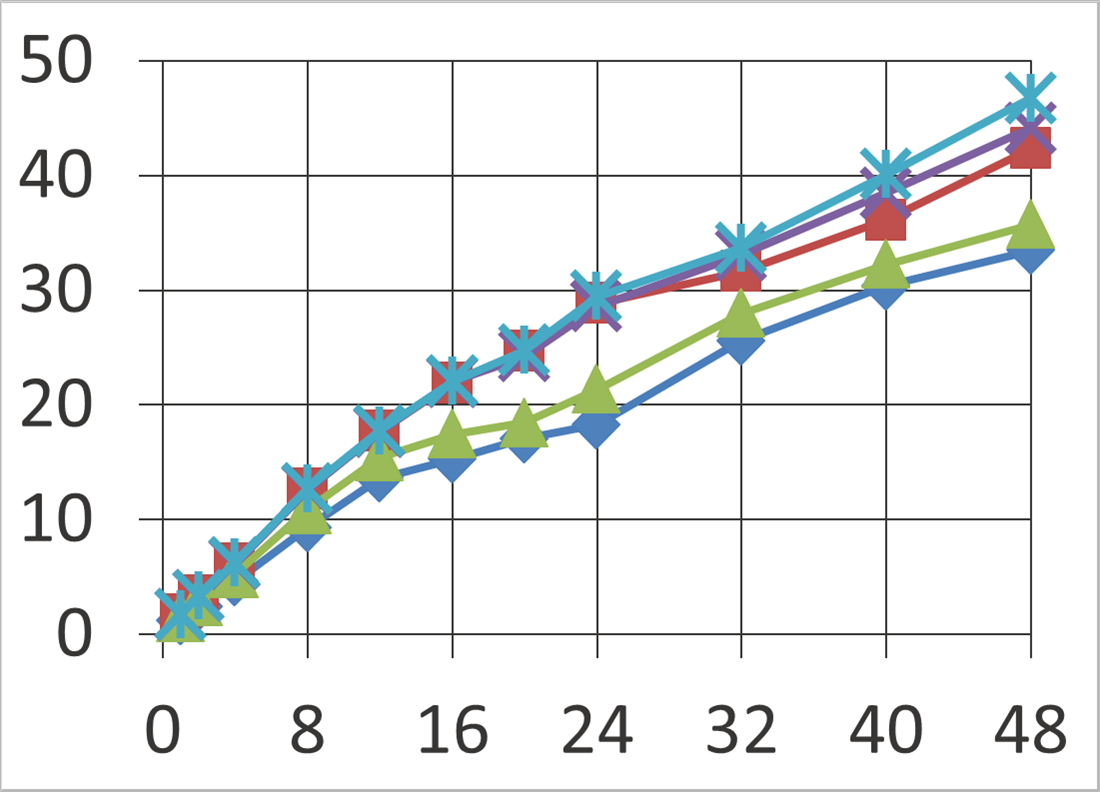
\includegraphics[width=\linewidth]{figures/graphs/0i0d100000k-nrq0.png} &
        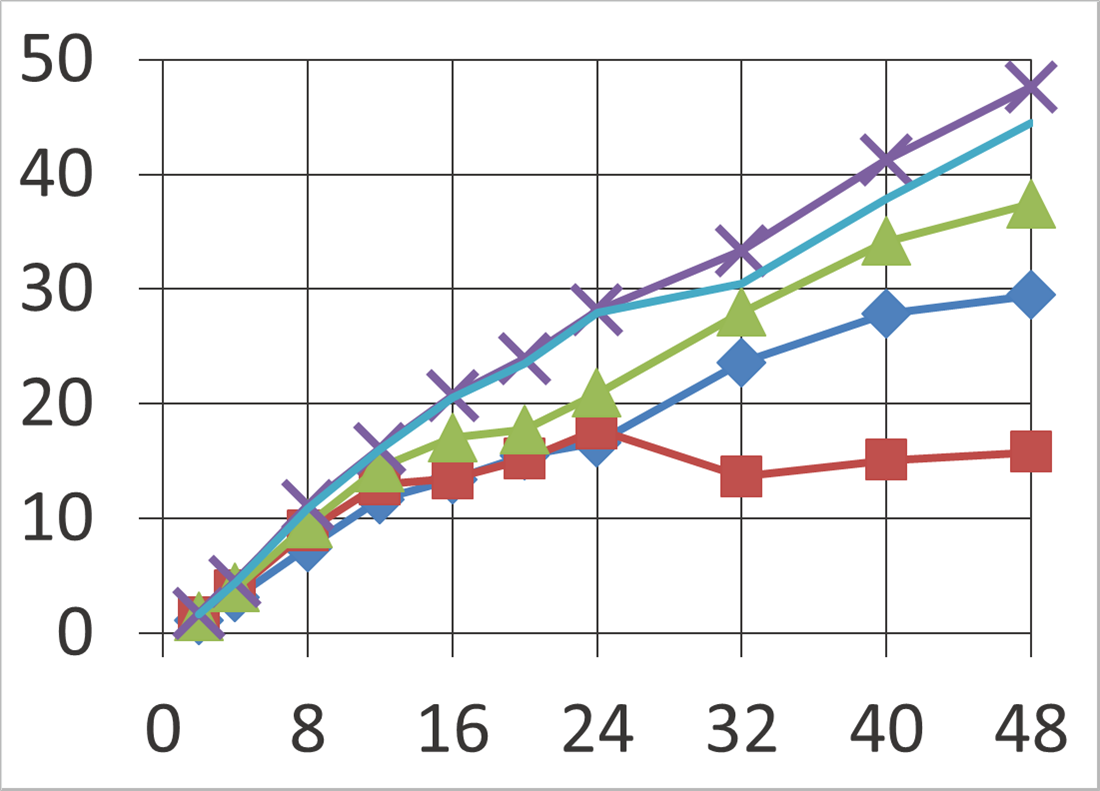
\includegraphics[width=\linewidth]{figures/graphs/0i0d100000k-nrq1.png}
        \\
        \vspace{-5mm}\rotatebox{90}{\small 10\% updates} &
        \vspace{-5mm}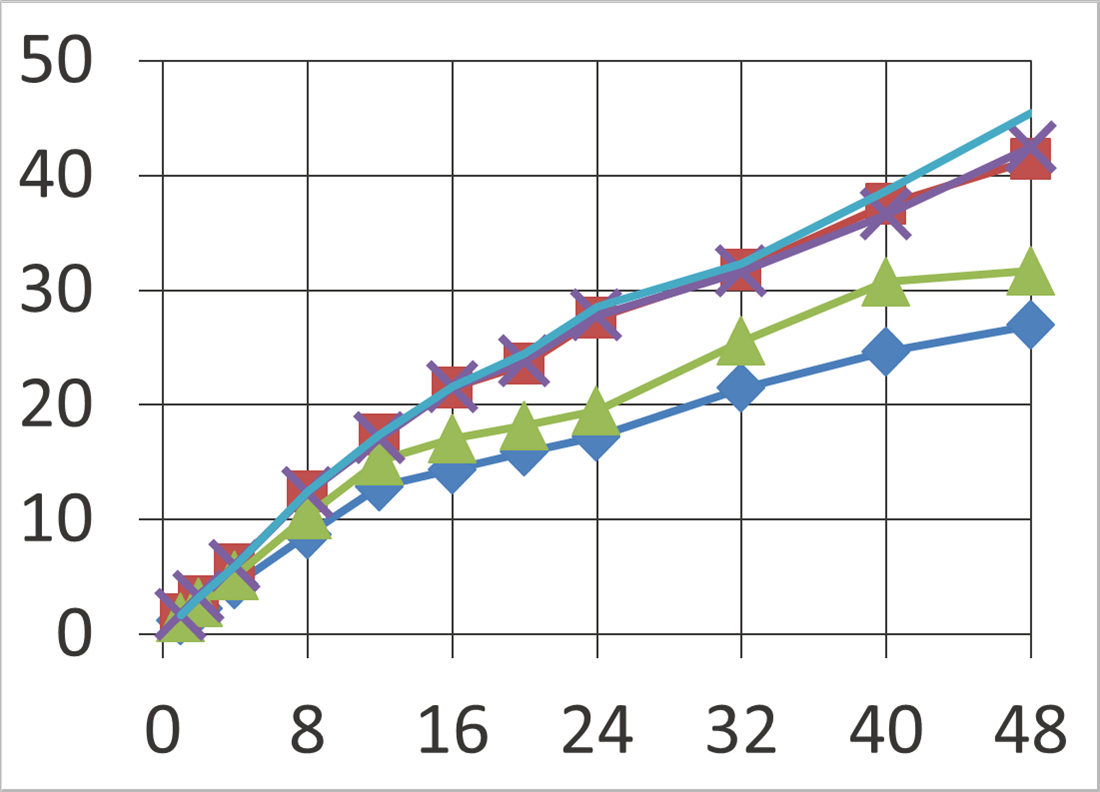
\includegraphics[width=\linewidth]{figures/graphs/5i5d100000k-nrq0.png} &
        \vspace{-5mm}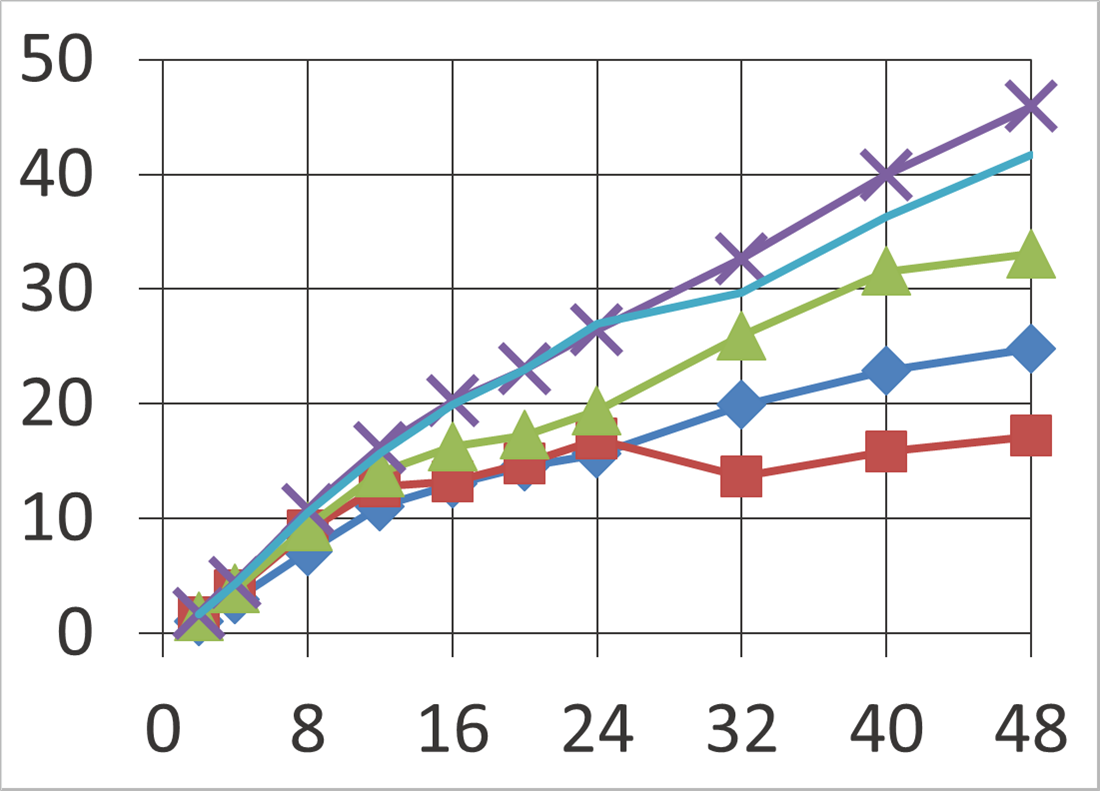
\includegraphics[width=\linewidth]{figures/graphs/5i5d100000k-nrq1.png}
        \\
        \vspace{-5mm}\rotatebox{90}{\small 40\% updates} &
        \vspace{-5mm}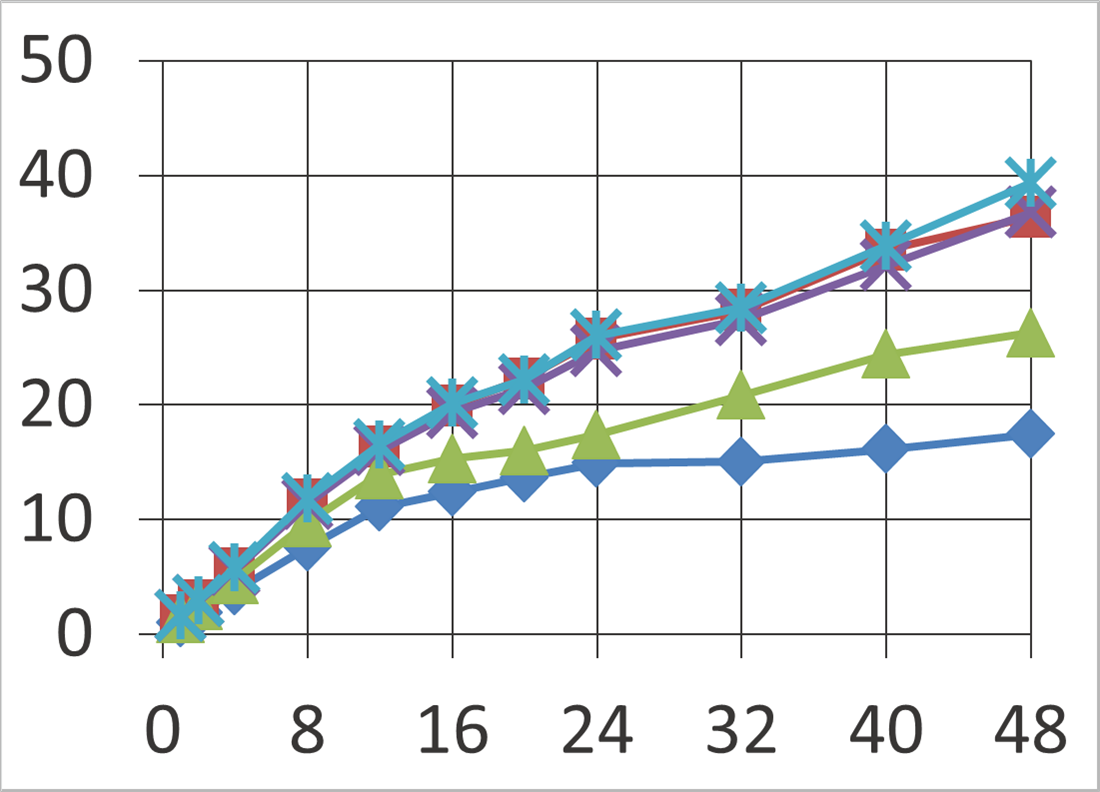
\includegraphics[width=\linewidth]{figures/graphs/20i20d100000k-nrq0.png} &
        \vspace{-5mm}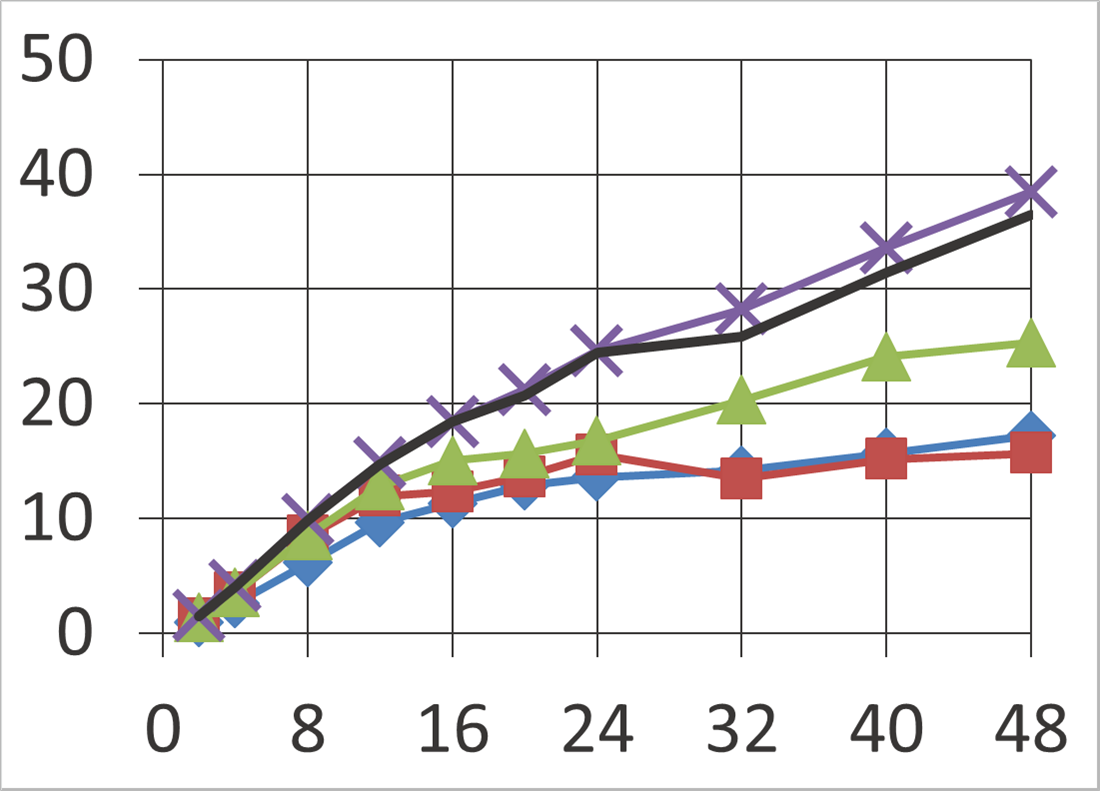
\includegraphics[width=\linewidth]{figures/graphs/20i20d100000k-nrq1.png}
        \\
    \end{tabular}
\end{minipage}
\begin{minipage}{0.495\linewidth}
    \centering
    \textbf{2x12-core IBM POWER8}
    \begin{tabular}{m{0.04\linewidth}m{0.48\linewidth}m{0.48\linewidth}}
        &
        \fcolorbox{black!50}{black!20}{\parbox{\dimexpr \linewidth-2\fboxsep-2\fboxrule}{\centering {\footnotesize No threads perform \textit{RangeIncrement} (W1)}}} &
        \fcolorbox{black!50}{black!20}{\parbox{\dimexpr \linewidth-2\fboxsep-2\fboxrule}{\centering {\footnotesize One thread performs \textit{RangeIncrement} (W2)}}}
        \\
        \rotatebox{90}{\small 0\% updates} &
        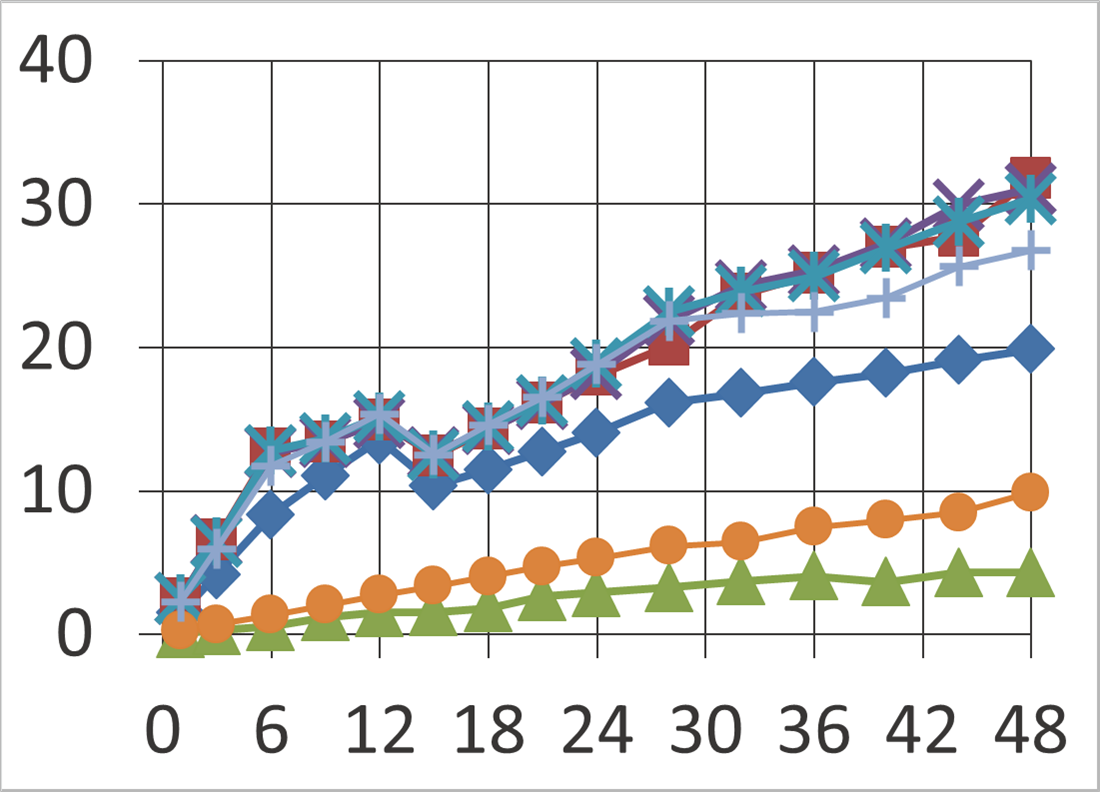
\includegraphics[width=\linewidth]{figures/graphs/power8/0i0d10000k-nrq0.png} &
        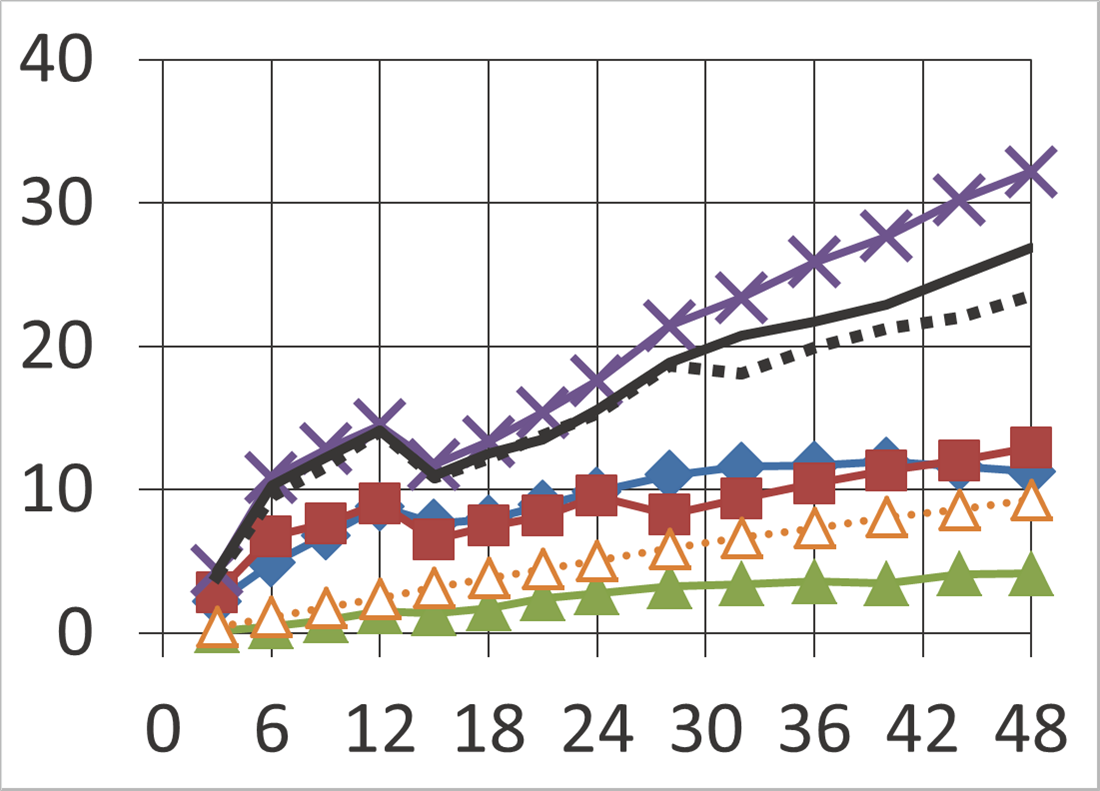
\includegraphics[width=\linewidth]{figures/graphs/power8/0i0d10000k-nrq1.png}
        \\
        \vspace{-5mm}\rotatebox{90}{\small 10\% updates} &
        \vspace{-5mm}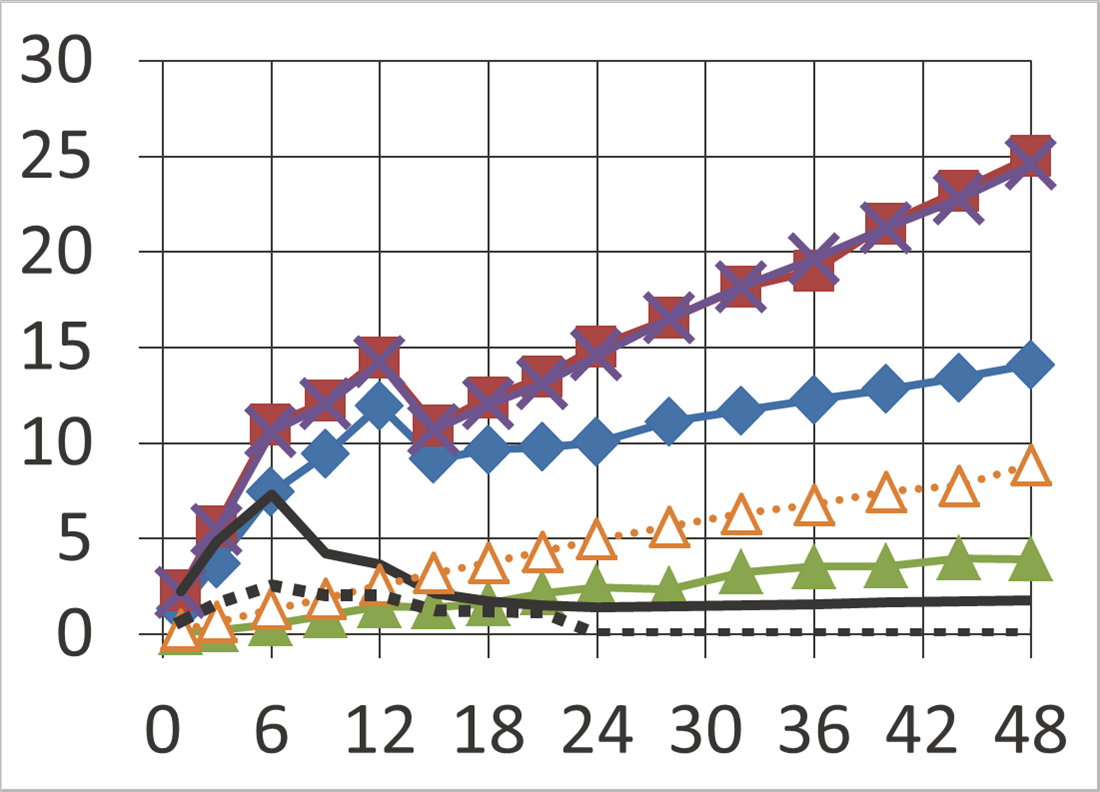
\includegraphics[width=\linewidth]{figures/graphs/power8/5i5d10000k-nrq0.png} &
        \vspace{-5mm}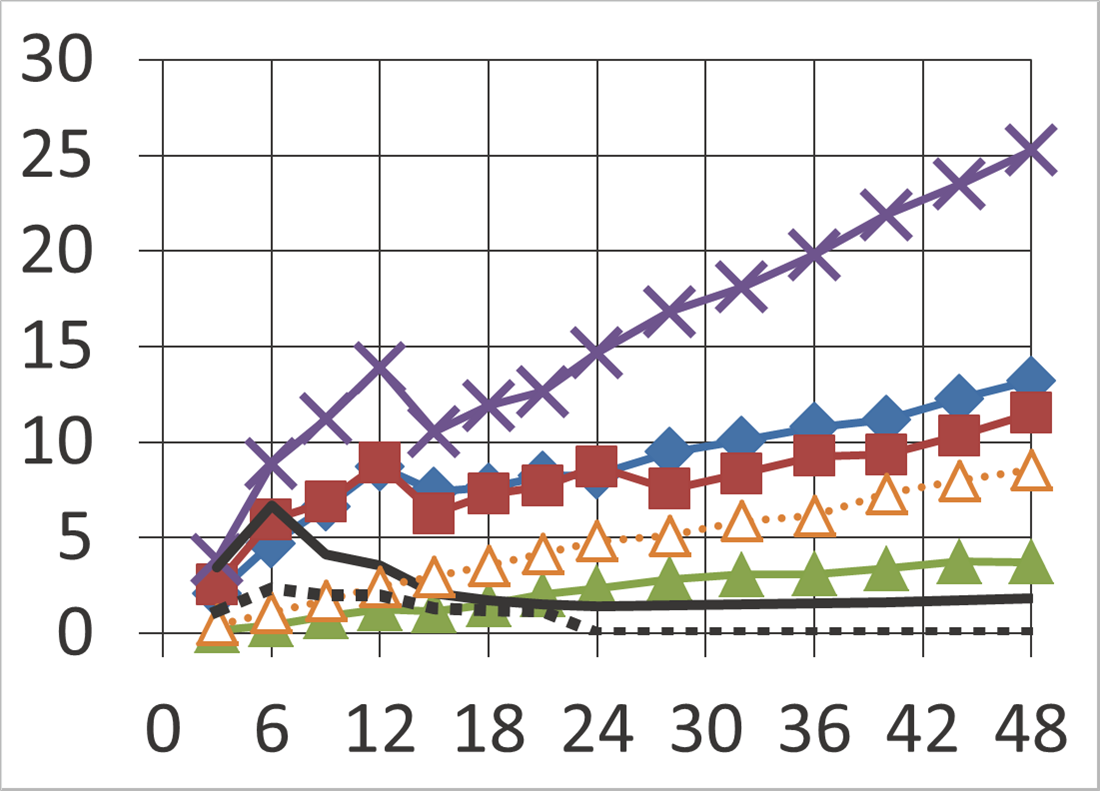
\includegraphics[width=\linewidth]{figures/graphs/power8/5i5d10000k-nrq1.png}
        \\
        \vspace{-5mm}\rotatebox{90}{\small 40\% updates} &
        \vspace{-5mm}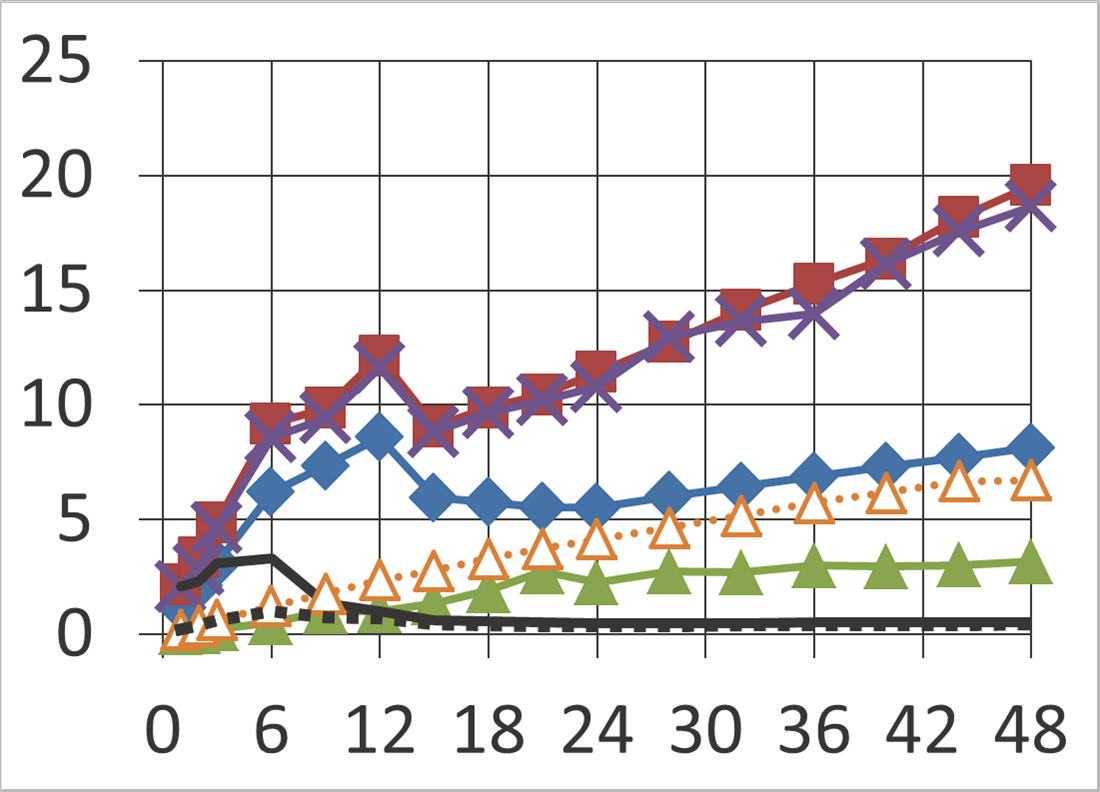
\includegraphics[width=\linewidth]{figures/graphs/power8/20i20d10000k-nrq0.png} &
        \vspace{-5mm}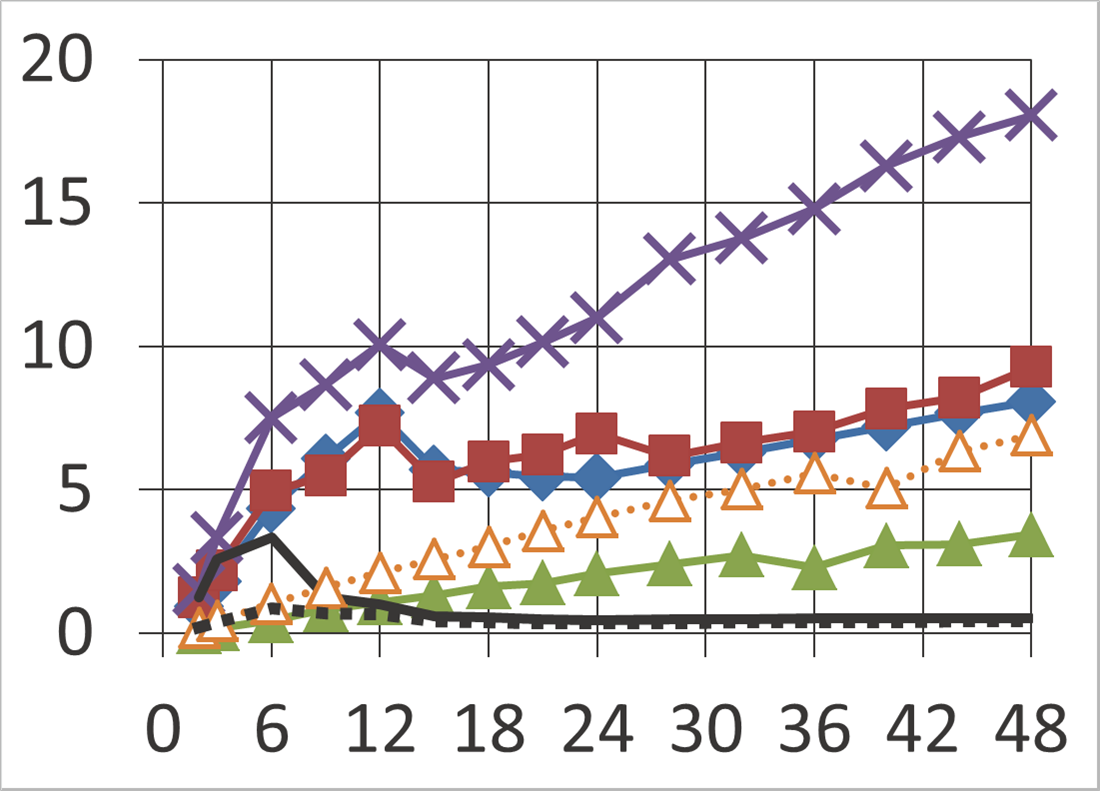
\includegraphics[width=\linewidth]{figures/graphs/power8/20i20d10000k-nrq1.png}
        \\
    \end{tabular}
\end{minipage}
    \vspace{-2mm}
	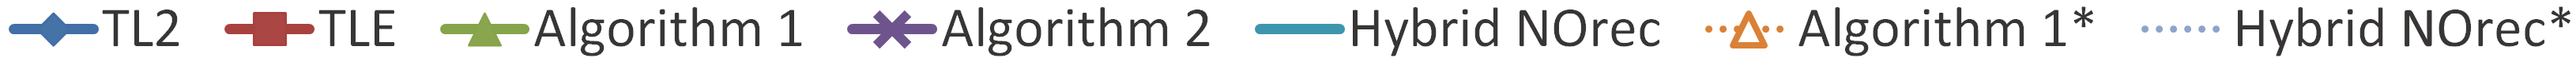
\includegraphics[width=\linewidth]{figures/graphs/power8/dsbench3_legend_power.png}
    \vspace{-4mm}
\caption{Results for a \textbf{BST microbenchmark}.
The x-axis represents the number of concurrent threads.
The y-axis represents operations per microsecond.}
\label{fig-exp-bst}
\end{figure}

\vspace{1mm}\noindent\textbf{Results (Intel).}
We first discuss the 0\% updates graph for workload type W1.
In this graph, essentially all operations committed in hardware.
In fact, in each trial, a small fraction of 1\% of operations ran on the slow-path.
Thus, any performance differences shown in the graph are essentially differences in the performance of the algorithms' respective fast-paths (with the exception of TL2).
Algorithm~\ref{alg:inswrite}, which has instrumentation in its fast-path read operations, has significantly lower performance than Algorithm~\ref{alg:inswrite2}, which does not.
Since this is a read-only workload, this instrumentation is responsible for the performance difference.

In the W1 workloads, TLE, Algorithm~\ref{alg:inswrite2} and Hybrid NOrec perform similarly (with a small performance advantage for Hybrid NOrec at high thread counts).
This is because the fast paths for these three algorithms have similar amounts of instrumentation: there is no instrumentation for reads or writes, 
and the transaction itself incurs one or two metadata accesses.
In contrast, in the W2 workloads, TLE performs quite poorly, compared to the HyTM algorithms.
In these workloads, transactions must periodically run on the slow-path, and in TLE, 
this entails acquiring a global lock that restricts progress for all other threads.
At high thread counts this significantly impacts performance.
Its performance decreases as the sizes of the ranges passed to \textit{RangeIncrement} increase.
Its performance is also negatively impacted by NUMA effects at thread counts higher than 24.
(This is because, when a thread $p$ reads the lock and incurs a cache miss, 
if the lock was last held by another thread on the same socket, 
then $p$ can fill the cache miss by loading it from the shared L3 cache.
However, if the lock was last held by a thread on a different socket, 
then $p$ must read the lock state from main memory, which is significantly more expensive.)
On the other hand, in each graph in the W2 workloads, the performance of each HyTM (and TL2) is similar to its performance in the corresponding W1 workload graph.
For Algorithm~\ref{alg:inswrite} (and TL2), this is because of progressiveness.
Although Algorithm~\ref{alg:inswrite2} is not truly progressive, fast-path transactions will abort only if they are concurrent with the commit procedure of a slow-path transaction.
In \textit{RangeIncrement} operations, there is a long read-only prefix (which is exceptionally long because of Algorithm~\ref{alg:inswrite2}'s quadratic validation) followed by a relatively small set of writes.
Thus, \textit{RangeIncrement} operations have relatively little impact on the fast-path.
The explanation is similar for Hybrid NOrec (except that it performs less validation than Algorithm~\ref{alg:inswrite2}).

Observe that the performance of Hybrid NOrec decreases slightly, relative to Algorithm~\ref{alg:inswrite2}, after 24 threads.
Recall that, in Hybrid NOrec, the global sequence number is a single point of contention on the fast-path.
(In Algorithm~\ref{alg:inswrite2}, the global lock is only modified by slow-path transactions, so fast-path transactions do not have a single point of contention.)
We believe this is due to NUMA effects, similar to those described in~\cite{BKLL16}.
Specifically, whenever a threads on the first socket performs a fast-path transaction that commits and modifies the global lock, it causes cache invalidations for all other threads.
Threads on socket two must then load the lock state from main memory, which takes much longer than loading it from the shared L3 cache.
This causes the transaction to run for a longer time, which lengthens its window of contention, making it more likely to abort.
(Note that, in the 0\% updates graph in the W2 workload, we still see this effect, because there is a thread performing \textit{RangeIncrement} operations.)
%% IF THIS DISCREPANCY IS DUE TO NUMA EFFECTS HURTING UPDATES, WHY DOES THE GAP BETWEEN ALGORITHMS DECREASE AS THE NUMBER OF UPDATES INCREASES?
% here's a subtle hypothesis. there are two different numa effects competing to be the dominating performance factor. one is the effect i just described above. the other is the negative performance impact of tree updates on traversals. this is something we saw in the oracle spaa paper when looking at tree updates in htm. i expect that the strength of the negative numa effects on tree traversals with increased updates is greater than the strength of the negative numa effects of esl and gsl updates. since the negative effects on tree traversals impact both algorithms, it makes the difference in performance less significant, masking the other numa effect.

\vspace{1mm}\noindent\textbf{Results (IBM POWER8).}
%
Algorithm~\ref{alg:inswrite} performs poorly on POWER8: POWER8 transactions can only load 64 cache lines before they will abort~\cite{nguyen-thesis}. 
Transactions read locks and tree nodes, which are in different cache lines: together, they often exceed 64 cache lines loaded in a tree operation, 
so most transactions cannot succeed in hardware. Consequently, on POWER8, 
it is incredibly important either to have minimal instrumentation in transactions, or for metadata to be located in the 
same cache lines as program data. Of course, the latter is not possible for HyTMs, which do not have control over the layout of program data.
Consequently, Algorithm~\ref{alg:inswrite2} outperforms Algorithm~\ref{alg:inswrite} in POWER8 quite easily by avoiding the per-read instrumentation. 

Algorithm~\ref{alg:inswrite} is improved slightly by the expensive (on POWER8) suspend/resume on sequence locks, so it still performs relatively poorly. 
To make suspend/resume a practical tool, one could imagine attempting to 
collect several metadata accesses and perform them together to amortize the cost of a suspend/resume pair. For instance, 
in Algorithm~\ref{alg:inswrite}, one might try to update the locks for all of a transactions writes at once, when the transaction commits. 
Typically one would accomplish this by logging all writes so that a process can remember which addresses it must lock at commit time. 
however, logging the writes inside the transaction would be at least as costly as just performing them.

Observe that Hybrid NOrec does far worse with updates in POWER8 than on the Intel machine.
This is due to the fact that fetch-increment on a single location experiences severe negative scaling on the Power8 processor: e.g., in one second, a single
thread can perform 37 fetch-add operations while 6 threads perform a total of 9 million and 24 threads perform only 4 million fetch-add operations.
In contrast, the Intel machine performs 32 million operations with 6 threads and 45 million with 24 threads. This is likely because this Intel processor provides 
fetch-add instructions while it must be emulated on the POWER8 processor.

In Hybrid NOrec\textsuperscript{$\ast$}, the non-speculative increment of gsl actually makes performance worse. Recall that in Hybrid NOrec, 
if a fast path transaction $T_1$ increments gsl, and then a software transaction $T_2$ reads gsl (as part of validation) before $T_1$ commits, then $T_1$ will abort, 
and $T_2$ will not see $T_1$'s change to gsl. 
So, $T_2$ will have a higher chance of avoiding incremental validation (and, hence, will likely take less time to run, and have a smaller contention window). 
However, in Hybrid NOrec\textsuperscript{$\ast$}, once $T_1$ increments gsl, $T_2$ will see the change to gsl, regardless of whether $T_1$ commits or aborts. Thus, 
$T_2$ will be forced to perform incremental validation. In our experiments, we observed that a much larger number of transactions ran on 
the fallback path in Hybrid NOrec\textsuperscript{$\ast$} than in Hybrid NOrec (often several orders of magnitude more).

%
%!TEX root = htm.tex
\section{Related work and discussion}
\label{sec:rel}
%
\paragraph{HyTM complexity.}
The proof of Theorem~\ref{th:impossibility} is heavily based on the analogous proof for step complexity of
STMs that are \emph{disjoint-access parallel} from \cite{prog15-pact}.
The model from \cref{sec:hytm} itself is an extension of the HyTM model introduced in \cite{hytm14disc}
which does not allow uncached accesses within the fast-path.

\paragraph{HyTM implementations.}
The HyTM implementation in \cite{damronhytm} uses the \emph{ROCK} processor~\cite{rock} as the underlying HTM
while \cite{kumarhytm} described a specific HTM design that requires the support of \emph{non-cached accesses}
within a hardware transaction. 
Recent work has investigated fallback to \emph{reduced} hardware transactions~\cite{MS13}
in which an all-software slow-path is replaced by a mix of hardware and software transactions. 
Afek \emph{et al}. proposed amalgamated lock elision (ALE)~\cite{ale15} which improves over TLE
by executing the slow-path as a series segments, each segment being a dynamic length hardware transaction.
The hybrid NOrec algorithm is described in \cite{hynorecriegel} which additionally proposed the use of non-speculative accesses
within fast-path transactions supported in the AMD ASF architectures.

\paragraph{Concluding remarks.}
In ongoing work, we are implementing our algorithms on the IBM Power8 HTM implementation which supports
non-cached accesses inside fast-path. We hope to understand if the instrumentation ovehead in
progressive HyTM implementations on Intel's HTM are also inherent to Power8's HTM implementation.
%
%!TEX root = htm.tex
\section{Concluding remarks}
\label{sec:conc}
%
\newpage
\bibliography{references2}
\appendix
%
%!TEX root = htm.tex
\section{Correctness proofs}
\label{app:proofs}
%
We will prove the opacity of Algorithm~\ref{alg:inswrite} even if some of accesses performed by fast-path transactions are direct (as indicated in the pseudocode).
Analogous arguments apply to Algorithm~\ref{alg:inswrite2}.
%
\begin{lemma}
\label{lm:opacityh1}
Algorithm~\ref{alg:inswrite} implements an opaque TM.
\end{lemma}
%
\begin{proof}
%
Let $E$ by any execution of Algorithm~\ref{alg:inswrite}. 
Since opacity is a safety property, it is sufficient to prove that every finite execution is opaque~\cite{icdcs-opacity}.
Let $<_E$ denote a total-order on events in $E$.

Let $H$ denote a subsequence of $E$ constructed by selecting
\emph{linearization points} of t-operations performed in $E$.
The linearization point of a t-operation $op$, denoted as $\ell_{op}$ is associated with  
a base object event or an event performed during 
the execution of $op$ using the following procedure. 

\vspace{1mm}\noindent\textbf{Completions.}
First, we obtain a completion of $E$ by removing some pending
invocations or adding responses to the remaining pending invocations
as follows:
%
\begin{itemize}
\item
incomplete $\Read_k$, $\Write_k$ operation performed by a slow-path transaction $T_k$ is removed from $E$;
an incomplete $\TryC_k$ is removed from $E$ if $T_k$ has not performed any write to a base object $r_j$; $X_j \in \Wset(T_k)$
in Line~\ref{line:write}, otherwise it is completed by including $C_k$ after $E$.
\item
every incomplete $\Read_k$, $\TryA_k$, $\Write_k$ and $\TryC_k$ performed by a fast-path transaction $T_k$ is removed from $E$.
\end{itemize}
%
\vspace{1mm}\noindent\textbf{Linearization points.}
Now a linearization $H$ of $E$ is obtained by associating linearization points to
t-operations in the obtained completion of $E$.
For all t-operations performed a slow-path transaction $T_k$, linearization points as assigned as follows:
%
\begin{itemize}
\item For every t-read $op_k$ that returns a non-A$_k$ value, $\ell_{op_k}$ is chosen as the event in Line~\ref{line:read2}
of Algorithm~\ref{alg:inswrite}, else, $\ell_{op_k}$ is chosen as invocation event of $op_k$
\item For every $op_k=\Write_k$ that returns, $\ell_{op_k}$ is chosen as the invocation event of $op_k$
\item For every $op_k=\TryC_k$ that returns $C_k$ such that $\Wset(T_k)
  \neq \emptyset$, $\ell_{op_k}$ is associated with the first write to a base object performed by $\lit{release}$
  when invoked in Line~\ref{line:rel}, 
  else if $op_k$ returns $A_k$, $\ell_{op_k}$ is associated with the invocation event of $op_k$
\item For every $op_k=\TryC_k$ that returns $C_k$ such that $\Wset(T_k) = \emptyset$, 
$\ell_{op_k}$ is associated with Line~\ref{line:return}
\end{itemize}
%
For all t-operations performed a fast-path transaction $T_k$, linearization points as assigned as follows:
\begin{itemize}
\item For every t-read $op_k$ that returns a non-A$_k$ value, $\ell_{op_k}$ is chosen as the event in Line~\ref{line:lin1}
of Algorithm~\ref{alg:inswrite}, else, $\ell_{op_k}$ is chosen as invocation event of $op_k$
\item
For every $op_k$ that is a $\TryC_k$, $\ell_{op_k}$ is the $\ms{commit-cache}_k$ primitive invoked by $T_k$
\item
For every $op_k$ that is a $\Write_k$, $\ell_{op_k}$ is the event in Line~\ref{line:lin2}.
\end{itemize}
%
$<_H$ denotes a total-order on t-operations in the complete sequential history $H$.

\vspace{1mm}\noindent\textbf{Serialization points.}
The serialization of a transaction $T_j$, denoted as $\delta_{T_j}$ is
associated with the linearization point of a t-operation 
performed by the transaction.

We obtain a t-complete history ${\bar H}$ from $H$ as follows. 
A serialization $S$ is obtained by associating serialization points to transactions in ${\bar H}$ as follows:
for every transaction $T_k$ in $H$ that is complete, but not t-complete, 
we insert $\textit{tryC}_k\cdot A_k$ immediately 
after the last event of $T_k$ in $H$. 
%
\begin{itemize}
\item If $T_k$ is an updating transaction that commits, then $\delta_{T_k}$ is $\ell_{\TryC_k}$
\item If $T_k$ is a read-only or aborted transaction,
then $\delta_{T_k}$ is assigned to the linearization point of the last t-read that returned a non-A$_k$ value in $T_k$
\end{itemize}
%
$<_S$ denotes a total-order on transactions in the t-sequential history $S$.
Since for a given transaction, its
serialization point is chosen between the first and last event of the transaction,
if $T_i \prec_{H} T_j$, then $\delta_{T_i} <_{E} \delta_{T_j}$ implies $T_i <_S T_j$.
%
\begin{claim}
\label{cl:alg1claim}
%
If process $p_i$ executing transaction $T_k\in \ms{txns}(E)$ holds the lock on $X_j\in \ms{Wset}(T_k)$ after $E$, then the value $r_j$ is an odd integer value.
\end{claim}
%
\begin{proof}
%
\end{proof}
%
\begin{claim}
\label{cl:readfrom}
$S$ is legal.
\end{claim}
%
\begin{proof}
%
We claim that for every $\Read_j(X_m) \rightarrow v$, there exists some slow-path transaction $T_i$ (or resp. fast-path)
that performs $\Write_i(X_m,v)$ and completes the event in Line~\ref{line:write} (or resp. Line~\ref{line:lin2}) such that
$\Read_j(X_m) \not\prec_H^{RT} \Write_i(X_m,v)$.

Suppose that $T_i$ is a slow-path transaction:
since $\Read_j(X_m)$ returns the response $v$, the event in Line~\ref{line:read2}
succeeds the event in Line~\ref{line:write} performed by $\TryC_i$. 
Since $\Read_j(X_m)$ can return a non-abort response only after $T_i$ writes $0$ to $r_m$ in
Line~\ref{line:rel1}, $T_i$ must be committed in $S$.
Consequently,
$\ell_{\TryC_i} <_E \ell_{\Read_j(X_m)}$.
Since, for any updating
committing transaction $T_i$, $\delta_{T_i}=\ell_{\TryC_i}$, it follows that
$\delta_{T_{i}} <_E \delta_{T_{j}}$.

Otherwise if $T_i$ is a fast-path transaction, then clearly $T_i$ is a committed transaction in $S$.
Recall that $\Read_j(X_m)$ can read $v$ during the event in Line~\ref{line:read2}
only after $T_i$ applies the $\ms{commit-cache}$ primitive.
By the assignment of linearization points, 
$\ell_{\TryC_i} <_E \ell_{\Read_j(X_m)}$ and thus, $\delta_{T_{i}} <_E \ell_{\Read_j(X_m)}$.

Thus, to prove that $S$ is legal, it suffices to show that  
there does not exist a
transaction $T_k$ that returns $C_k$ in $S$ and performs $\Write_k(X_m,v')$; $v'\neq v$ such that $T_i <_S T_k <_S T_j$. 
%

$T_i$ and $T_k$ are both updating transactions that commit. Thus, 
%
\begin{center}
($T_i <_S T_k$) $\Longleftrightarrow$ ($\delta_{T_i} <_{E} \delta_{T_k}$) \\
($\delta_{T_i} <_{E} \delta_{T_k}$) $\Longleftrightarrow$ ($\ell_{\TryC_i} <_{E} \ell_{\TryC_k}$) 
\end{center}
%
Since, $T_j$ reads the value of $X$ written by $T_i$, one of the following is true:
$\ell_{\TryC_i} <_{E} \ell_{\TryC_k} <_{E} \ell_{\Read_j(X_m)}$ or
$\ell_{\TryC_i} <_{E} \ell_{\Read_j(X_m)} <_{E} \ell_{\TryC_k}$.

Suppose that $\ell_{\TryC_i} <_{E} \ell_{\TryC_k} <_{E} \ell_{\Read_j(X_m)}$.

(\textit{Case \RNum{1}:}) $T_i$ and $T_k$ are slow-path transactions.

Thus, $T_k$ returns a response from the event in Line~\ref{line:acq} 
before the read of the base object associated with $X_m$ by $T_j$ in Line~\ref{line:read2}. 
Since $T_i$ and $T_k$ are both committed in $E$, $T_k$ returns \emph{true} from the event in
Line~\ref{line:acq} only after $T_i$ writes $0$ to $r_{m}$ in Line~\ref{line:rel1}.

If $T_j$ is a slow-path transaction, 
recall that $\Read_j(X_m)$ checks if $X_j$ is locked by a concurrent transaction, 
then performs read-validation (Line~\ref{line:abort0}) before returning a matching response. 
We claim that $\Read_j(X_m)$ must return $A_j$ in any such execution.

Consider the following possible sequence of events: 
$T_k$ returns \emph{true} from \emph{acquire} function invocation, 
updates the value of $X_m$ to shared-memory (Line~\ref{line:write}), 
$T_j$ reads the base object $v_m$ associated with $X_m$, 
$T_k$ releases $X_m$ by writing $0$ to $r_{m}$ and finally $T_j$ performs the check in Line~\ref{line:abort0}. 
But in this case, $\Read_j(X_m)$ is forced to return the value $v'$ written by $T_m$--- 
contradiction to the assumption that $\Read_j(X_m)$ returns $v$. 

Otherwise suppose that $T_k$ acquires exclusive access to $X_m$ by writing $1$ to $r_{m}$ and returns \emph{true}
from the invocation of \emph{acquire}, updates $v_m$ in Line~\ref{line:write}), 
$T_j$ reads $v_m$, $T_j$ performs the check in Line~\ref{line:abort0} and finally $T_k$ 
releases $X_m$ by writing $0$ to $r_{m}$. 
Again, $\Read_j(X_m)$ must return $A_j$ since $T_j$ reads that $r_{m}$ is $1$---contradiction.

A similar argument applies to the case that $T_j$ is a fast-path transaction.
Indeed, since every \emph{data} base object read by $T_j$ is contained in its tracking set, if any concurrent
transaction updates any t-object in its read set, $T_j$ is aborted immediately by our model(cf. Section~\ref{sec:hytm}).

Thus, $\ell_{\TryC_i} <_E \ell_{\Read_j(X)} <_{E} \ell_{\TryC_k}$.

(\textit{Case \RNum{2}:}) $T_i$ is a slow-path transaction and $T_k$ is a fast-path transaction.
Thus, $T_k$ returns $C_k$ 
before the read of the base object associated with $X_m$ by $T_j$ in Line~\ref{line:read2}, but after the response
of \emph{acquire} by $T_i$ in Line~\ref{line:acq}.
Since $\Read_j(X_m)$ reads the value of $X_m$ to be $v$ and not $v'$, $T_i$ performs the \emph{cas}
to $v_m$ in Line~\ref{line:write} after the $T_k$ performs the $\ms{commit-cache}$ primitive (since if
otherwise, $T_k$ would be aborted in $E$).
But then the \emph{cas} on $v_m$ performed by $T_i$ would return $\false$ and $T_i$ would return $A_i$---contradiction.

(\textit{Case \RNum{3}:}) $T_k$ is a slow-path transaction and $T_i$ is a fast-path transaction.
This is analogous to the above case.

(\textit{Case \RNum{4}:}) $T_i$ and $T_k$ are fast-path transactions.
Thus, $T_k$ returns $C_k$ 
before the read of the base object associated with $X_m$ by $T_j$ in Line~\ref{line:read2}, but before $T_i$
returns $C_i$ (this follows from Observation).
Consequently, $\Read_j(X_m)$ must read the value of $X_m$ to be $v'$ and return $v'$---contradiction.
%

We now need to prove that $\delta_{T_{j}}$ indeed precedes $\ell_{\TryC_k}$ in $E$.

Consider the two possible cases:
%
\begin{itemize}
\item
Suppose that $T_j$ is a read-only transaction. 
Then, $\delta_{T_j}$ is assigned to the last t-read performed by $T_j$ that returns a non-A$_j$ value. 
If $\Read_j(X_m)$ is not the last t-read that returned a non-A$_j$ value, then there exists a $\Read_j(X')$ such that 
$\ell_{\Read_j(X_m)} <_{E} \ell_{\TryC_k} <_E \ell_{read_j(X')}$.
But then this t-read of $X'$ must abort by performing the checks in Line~\ref{line:abort0} or incur a tracking set abort---contradiction.
\item
Suppose that $T_j$ is an updating transaction that commits, then $\delta_{T_j}=\ell_{\TryC_j}$ which implies that
$\ell_{read_j(X)} <_{E} \ell_{\TryC_k} <_E \ell_{\TryC_j}$. Then, $T_j$ must neccesarily perform the checks
in Line~\ref{line:abort3} and return $A_j$ or incur a tracking set abort---contradiction to the assumption that $T_j$ is a committed transaction.
\end{itemize}
%
The proof follows.
%
\end{proof}
%
Since $S$ is legal and respects the real-time ordering of transactions, Algorithm~\ref{alg:inswrite} is opaque.
%
\end{proof}
%

\end{document}
%%% Local Variables:
%%% mode: latex
%%% mode: flyspell
%%% Local IspellDict: "american"
%%% mode: outline-minor
%%% End:

